\documentclass[11pt]{article}

% arXiv-style preprint layout
\usepackage[T1]{fontenc}
\usepackage[utf8]{inputenc}
\usepackage{lmodern}
\usepackage{microtype}
\usepackage[margin=1in]{geometry}
\usepackage{graphicx}
\usepackage{booktabs}
\usepackage{multirow}
\usepackage{amsmath}
\usepackage{xcolor}
\usepackage{tikz}
\usetikzlibrary{positioning,arrows.meta,fit,backgrounds}
\usepackage[font=small,labelfont=bf]{caption}
\usepackage{enumitem}
\usepackage{float}
\usepackage{fancyhdr}
\usepackage[numbers,sort&compress]{natbib}
\usepackage[colorlinks=true,linkcolor=blue!50!black,citecolor=blue!50!black,urlcolor=blue!50!black]{hyperref}

\graphicspath{{figures/}{../results/}}
% \input is not expandable inside tabular; the TeX primitive is
\makeatletter\newcommand{\inputrows}[1]{\@@input #1 }\makeatother
\definecolor{gemma}{HTML}{0F4D92}
\definecolor{qwen}{HTML}{42949E}
\setlist{itemsep=2pt,topsep=4pt}

\pagestyle{fancy}
\fancyhf{}
\renewcommand{\headrulewidth}{0pt}
\fancyhead[C]{\small\textit{Preprint}}
\fancyfoot[C]{\thepage}

\newcommand{\Gm}{Gemma~4 E2B}
\newcommand{\Qw}{Qwen3.5-4B}
\newcommand{\fileone}{File@1}
\newcommand{\filefive}{File@5}
\newcommand{\funcfive}{Function@5}

\title{\textbf{Grammar Matters More Than Graphs:\\ Training-Free Bug Localization with Sub-4B Language Models\\ on a 4\,GB Consumer GPU}}
\author{Yukteswar\\[2pt]
  \small\url{https://github.com/yukteswar23/slm-bug-localizer}}
\date{November 2026}

\begin{document}
\maketitle
\thispagestyle{fancy}

\begin{abstract}
\noindent
We ask how far scaffolding alone can push off-the-shelf language models of at most 4B parameters at \emph{bug localization}, finding the files and functions that a GitHub issue requires to change, when the models run fully offline on a laptop with a 4\,GB GPU and receive no training.
We build one ReAct-style agent harness with file tools, code-graph tools, an Evidence Buffer, behavioural guards and grammar-constrained decoding, and ablate it on SWE-bench Lite with two model families, \Gm{} and \Qw{} (4-bit, llama.cpp).
Over 1{,}000 test episodes (100 tasks $\times$ 5 configurations $\times$ 2 models, 13.3 GPU-hours) and a 23-task development split, we find:
(i)~grammar-constrained decoding is the single most important component; removing it costs \Qw{} 46 points of \fileone{} (85\%\,$\to$\,39\%; 46 tasks lost, none gained, exact McNemar $p<10^{-13}$), mostly because the model drops the tool name from its final answer;
(ii)~the \emph{form} of the answer matters as much as the search: a structured answer format, a repeated-call guard, budget hints and ranked lists raise \Qw{}'s \funcfive{} from 51\% to 70\% (17 tasks gained, 0 lost, $p<10^{-4}$), while a regex-forced format halves accuracy on the development split by corrupting correct answers;
(iii)~code-graph tools and an Evidence Buffer give no significant gain; the models route under 12\% of calls to the graph tools, and the buffer adds 17--27\% generated tokens.
The best configuration (\Qw{}, C2) reaches 85\% \fileone{} and 74\% \funcfive{} at about 45\,s per task, against 33\% and 36\% for BM25 retrieval.
\Gm{} benefits from the harness in behaviour (forced answers fall from 72\% to 9\%) but not in accuracy, and at function level does not beat BM25.
Code, per-task results and all figures are public.
\end{abstract}

% ======================================================================
\section{Introduction}
\label{sec:intro}

Coding agents built on large language models (LLMs) now resolve a substantial share of real GitHub issues~\cite{jimenez2024swebench,yang2024sweagent,xia2024agentless}.
Most of this progress relies on frontier models served through APIs.
A practical first step of every issue-resolution pipeline, however, is \emph{localization}: deciding which files and functions must change.
Localization is cheaper to evaluate than repair, useful on its own (for triage, code review and developer navigation), and it is the step most likely to be feasible for small models running locally, where source code never leaves the machine.

This paper studies localization under tight constraints: models of at most 4B parameters, quantized to 4 bits, served by llama.cpp on a laptop GPU with 4\,GB of memory, with no fine-tuning.
Instead of changing the model, we change the \emph{scaffolding}, the harness around it, and ask which parts of a typical agent design actually help small models.
We test four hypotheses, fixed before the test runs:
\begin{itemize}
\item[\textbf{H1}] Each scaffolding component (harness fixes, code-graph tools, an Evidence Buffer) improves localization over a plain ReAct agent with file tools.
\item[\textbf{H2}] Grammar-constrained tool calls are essential for small models: invalid tool calls are a major failure mode below 4B.
\item[\textbf{H3}] The gains hold across model families (Gemma, Qwen).
\item[\textbf{H4}] Fixing remains far harder than localization at this scale (planned as a secondary experiment).
\end{itemize}

\paragraph{Contributions.}
\begin{enumerate}
\item A fully offline localization agent for a 4\,GB GPU, with grammar-constrained decoding through llama.cpp, and an evaluation harness with paired statistics; all code and per-task results are released (Section~\ref{sec:setup}).
\item A component-by-component ablation on 100 SWE-bench Lite test tasks and a 23-task development split, for two model families, with exact McNemar tests on paired outcomes (Sections~\ref{sec:dev}--\ref{sec:test}).
\item Evidence that for small models the decisive components are the ones that control the \emph{output}: grammar-constrained decoding and the answer format. Search-side additions popular for large models (graph tools, memory buffers) do not help, largely because small models do not use them (Section~\ref{sec:discussion}).
\item A negative result on format constraints: a regex grammar can guarantee the form of an answer while destroying its content, when the forced form diverges from the form the model is already writing (Section~\ref{sec:dev-format}).
\end{enumerate}

% ======================================================================
\section{Related work}
\label{sec:related}

\paragraph{Issue resolution and localization.}
SWE-bench~\cite{jimenez2024swebench} collects real GitHub issues with their fixing patches; SWE-bench Lite is a 300-task subset of self-contained issues.
Agent systems such as SWE-agent~\cite{yang2024sweagent} and AutoCodeRover~\cite{zhang2024autocoderover} interleave tool use and reasoning (in the style of ReAct~\cite{yao2023react}), while Agentless~\cite{xia2024agentless} shows that a fixed localize-then-repair pipeline is competitive.
LocAgent~\cite{chen2025locagent} represents the repository as a code graph and lets an LLM agent traverse it, reporting strong file- and function-level localization.
All of these use large models; we ask which of their ingredients transfer to models below 4B parameters on consumer hardware.

\paragraph{Constrained decoding.}
Grammar-constrained decoding restricts sampling to strings accepted by a grammar or JSON schema~\cite{geng2023grammar,willard2023outlines}, guaranteeing parseable tool calls.
\citet{tam2024speak} report that strict format restrictions can reduce reasoning accuracy.
Our development experiments show a related but distinct failure: a constraint that disagrees with the format the model is mid-way through writing corrupts the content of the answer (Section~\ref{sec:dev-format}).

\paragraph{Retrieval baselines.}
BM25~\cite{robertson2009bm25} over code is the standard non-neural baseline for localization; we use it as configuration C0.

% ======================================================================
\section{Setup}
\label{sec:setup}

\subsection{Task, data and metrics}
Given an issue text and the repository at the issue's base commit, the agent must submit a ranked list of files and a ranked list of functions to edit.
Gold locations come from the reference patch: every changed file, and the innermost function or method enclosing each changed line of an existing Python file (parsed with Python's \texttt{ast}).

\paragraph{Splits.} We tune on the official SWE-bench Lite \emph{dev} split (23 tasks from 6 repositories that do not appear in the test split) and evaluate once on a fixed 100-task subset of the 300-task \emph{test} split, sampled with a fixed seed and stratified by repository (12 repositories; django 38, sympy 26, matplotlib 8, scikit-learn 8, pytest 6, sphinx 5, others $\le$2).
The subset was fixed before any test run.
Every gold patch in the subset touches a single file; 12 tasks change no existing function (module-level code or new files) and are excluded from function metrics, leaving $n=88$.

\paragraph{Metrics.} \textbf{File@$k$}: every gold file is among the top-$k$ submitted files. \textbf{Function@$k$}: every gold function is among the top-$k$ submitted functions (a method also matches when the model omits its class prefix; module-style paths such as \texttt{pkg.mod} are normalised to \texttt{pkg/mod.py}). We report 95\% Wilson intervals and compare configurations with exact McNemar tests on paired per-task outcomes. We also record behavioural metrics: forced submissions (the model answered only because the final turn allowed nothing else), repeated identical calls, invalid replies, empty answers, steps, generated tokens and wall time.

\subsection{Models and hardware}
\label{sec:hardware}
We use \Gm{} (Google's quantization-aware Q4\_0 release, about 2B effective parameters) and \Qw{} (Q4\_K\_M), both in non-thinking mode, served by llama.cpp (\texttt{llama-server}, build b11873, CUDA) with all layers on the GPU, flash attention, a 12{,}288-token context and a single slot, so the prompt prefix stays in the KV cache between steps.
Decoding is greedy (temperature 0, seed 0).
The machine is a laptop with an NVIDIA RTX 2050 (4\,GB), 14\,GB RAM and a Ryzen 5 5500H.
Figure~\ref{fig:hw} shows that both models fit on the GPU: at 6K tokens of existing context, \Gm{} generates about 58 tokens/s using 2.1\,GB, and \Qw{} about 31 tokens/s using up to 3.7\,GB.
Because generation is slow, thinking mode is disabled; every generated token costs roughly 20--30\,ms.

\begin{figure}[t]
\centering
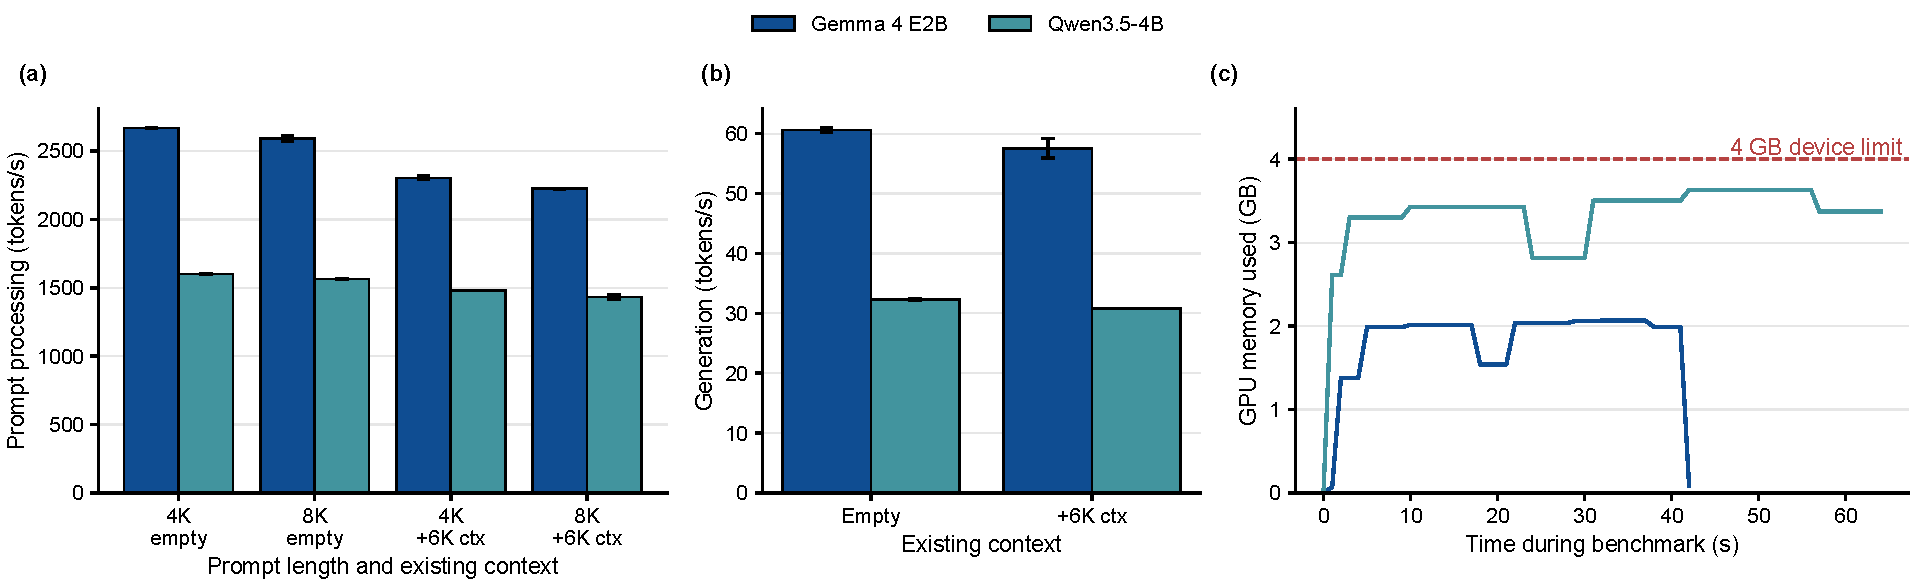
\includegraphics[width=\textwidth]{2026-10-25_01_hw-bench/figures/hw_bench.pdf}
\caption{\textbf{Hardware benchmark} (\texttt{llama-bench}, 2 repetitions, error bars: range). (a)~Prompt processing and (b)~generation throughput on an empty context and after 6K tokens of context. (c)~GPU memory during the benchmark; both models stay under the 4\,GB device limit.}
\label{fig:hw}
\end{figure}

\subsection{Agent harness}
Figure~\ref{fig:overview} shows the harness.
Each turn the model returns one JSON object \texttt{\{"thought": ..., "action": \{"tool": ..., args\}\}}.
The system prompt lists the tools; the issue is truncated to 6{,}000 characters; every tool output is capped at 4{,}000 characters (about 1K tokens); when the conversation exceeds 22{,}000 characters (about 6K tokens), the oldest tool outputs are replaced by one-line stubs.
Episodes have 20 turns; on the last turn only \texttt{submit} is allowed, so every episode ends with an answer.

\begin{figure}[t]
\centering
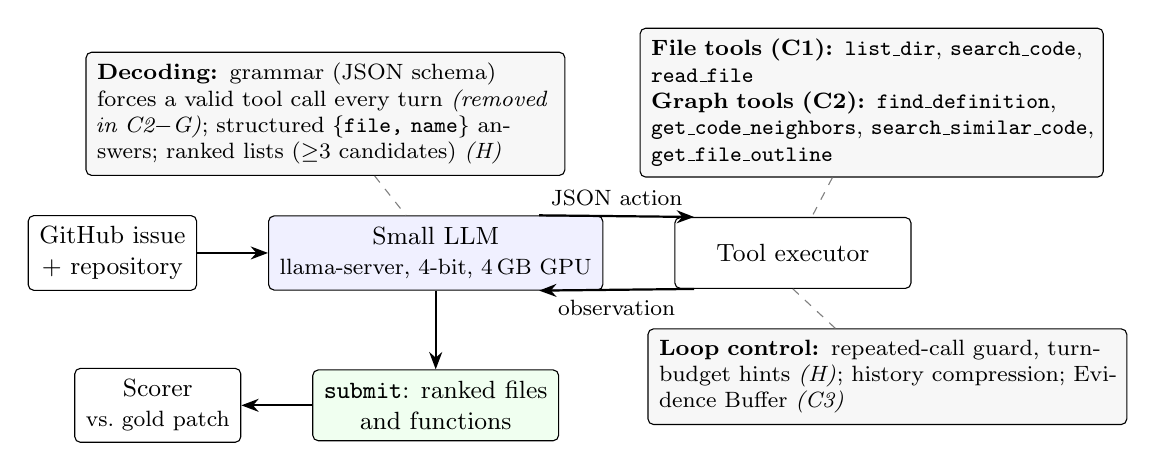
\begin{tikzpicture}[
  node distance=6mm and 9mm,
  box/.style={draw, rounded corners=2pt, align=center, font=\small, minimum height=9mm, inner sep=4pt, fill=white},
  comp/.style={draw, rounded corners=2pt, align=left, font=\footnotesize, inner sep=4pt, fill=gray!6},
  arr/.style={-{Stealth[length=2.2mm]}, thick}]
\node[box] (issue) {GitHub issue\\ + repository};
\node[box, right=of issue, fill=blue!6, minimum width=36mm] (llm) {Small LLM\\ \footnotesize llama-server, 4-bit, 4\,GB GPU};
\node[box, right=of llm, minimum width=30mm] (tools) {Tool executor};
\node[box, below=10mm of llm, fill=green!6] (submit) {\texttt{submit}: ranked files\\ and functions};
\node[box, left=of submit] (score) {Scorer\\ \footnotesize vs.\ gold patch};
\draw[arr] (issue) -- (llm);
\draw[arr] (llm.20) -- node[above, font=\footnotesize] {JSON action} (tools.160);
\draw[arr] (tools.200) -- node[below, font=\footnotesize] {observation} (llm.340);
\draw[arr] (llm) -- (submit);
\draw[arr] (submit) -- (score);
\node[comp, above=5mm of llm, xshift=-14mm, text width=58mm] (dec) {\textbf{Decoding:} grammar (JSON schema) forces a valid tool call every turn \emph{(removed in C2$-$G)}; structured \texttt{\{file, name\}} answers; ranked lists ($\ge$3 candidates) \emph{(H)}};
\node[comp, above=5mm of tools, xshift=10mm, text width=56mm] (tl) {\textbf{File tools (C1):} \texttt{list\_dir}, \texttt{search\_code}, \texttt{read\_file}\\ \textbf{Graph tools (C2):} \texttt{find\_definition}, \texttt{get\_code\_neighbors}, \texttt{search\_similar\_code}, \texttt{get\_file\_outline}};
\node[comp, below=5mm of tools, xshift=12mm, text width=58mm] (ctl) {\textbf{Loop control:} repeated-call guard, turn-budget hints \emph{(H)}; history compression; Evidence Buffer \emph{(C3)}};
\draw[dashed, gray] (dec) -- (llm);
\draw[dashed, gray] (tl) -- (tools);
\draw[dashed, gray] (ctl) -- (tools.south);
\end{tikzpicture}
\caption{\textbf{Agent harness.} The model alternates tool calls and observations for up to 20 turns, then submits ranked files and functions. Components are switched on cumulatively by the configurations in Table~\ref{tab:configs}.}
\label{fig:overview}
\end{figure}

\paragraph{Components.}
\begin{itemize}
\item \textbf{Grammar-constrained decoding.} The reply schema (tool name plus the tool's arguments, with bounded string patterns) is compiled by llama.cpp into a grammar that holds from the first token. Requests go through \texttt{/apply-template} and \texttt{/completion}: the chat endpoint applied the grammar only after a thinking block, which \Gm{} opened on its own, producing invalid replies.
\item \textbf{Harness fixes (H)}, four changes found on the dev split (Section~\ref{sec:dev}): a \emph{structured answer} in which each function is an object \texttt{\{"file", "name"\}}; a \emph{repeated-call guard} that refuses an exact repeat of an earlier call and tells the model to act differently or submit; \emph{budget hints} (\texttt{[Turn $i$ of 20]}, and in the last five turns ``submit as soon as you have a candidate''); and \emph{ranked lists} (\texttt{submit} requires 3--5 files and 3--10 functions, best first).
\item \textbf{Graph tools (C2)} over an \texttt{ast} index of the repository: definition lookup, a name-matched call graph (callers and callees), BM25 search over function bodies, and file outlines.
\item \textbf{Evidence Buffer (C3)}: each reply carries a required \texttt{evidence} field (at most 200 characters); collected facts are appended to the latest observation, and old outputs are hidden in one chunk so that the prompt prefix, and thus the KV cache, changes less often.
\end{itemize}

\begin{table}[t]
\centering
\small
\caption{\textbf{Configurations.} Each row adds one component to the row above; C2$-$G removes grammar-constrained decoding from C2.}
\label{tab:configs}
\begin{tabular}{lll}
\toprule
ID & Configuration & Notes \\
\midrule
C0 & BM25 retrieval, no LLM & files ranked by issue--file BM25; functions ranked within the top-5 files \\
C1 & ReAct agent + file tools & free-form function names, no guards \\
C1+H & C1 + harness fixes & structured answers, repeat guard, budget hints, ranked lists \\
C2 & C1+H + graph tools & best configuration on the dev split (``full system'') \\
C3 & C2 + Evidence Buffer & \\
C2$-$G & C2 without grammar & replies parsed from free text; parse failures count as invalid steps \\
\bottomrule
\end{tabular}
\end{table}

% ======================================================================
\section{Development experiments}
\label{sec:dev}

All harness decisions were made on the 23-task dev split, in the order below; Table~\ref{tab:dev} summarises them, and Appendix~\ref{app:figures} has the per-experiment figures.

\paragraph{Smoke test.}
A single task end to end (Figure~\ref{fig:smoke}) exposed two engineering problems that shaped the harness: the chat endpoint's lazy grammar (fixed by \texttt{/completion}, giving 0 invalid replies), and the cost of history compression, which changes the prompt prefix so that later steps reprocess about 6K tokens instead of reusing the KV cache.

\begin{figure}[t]
\centering
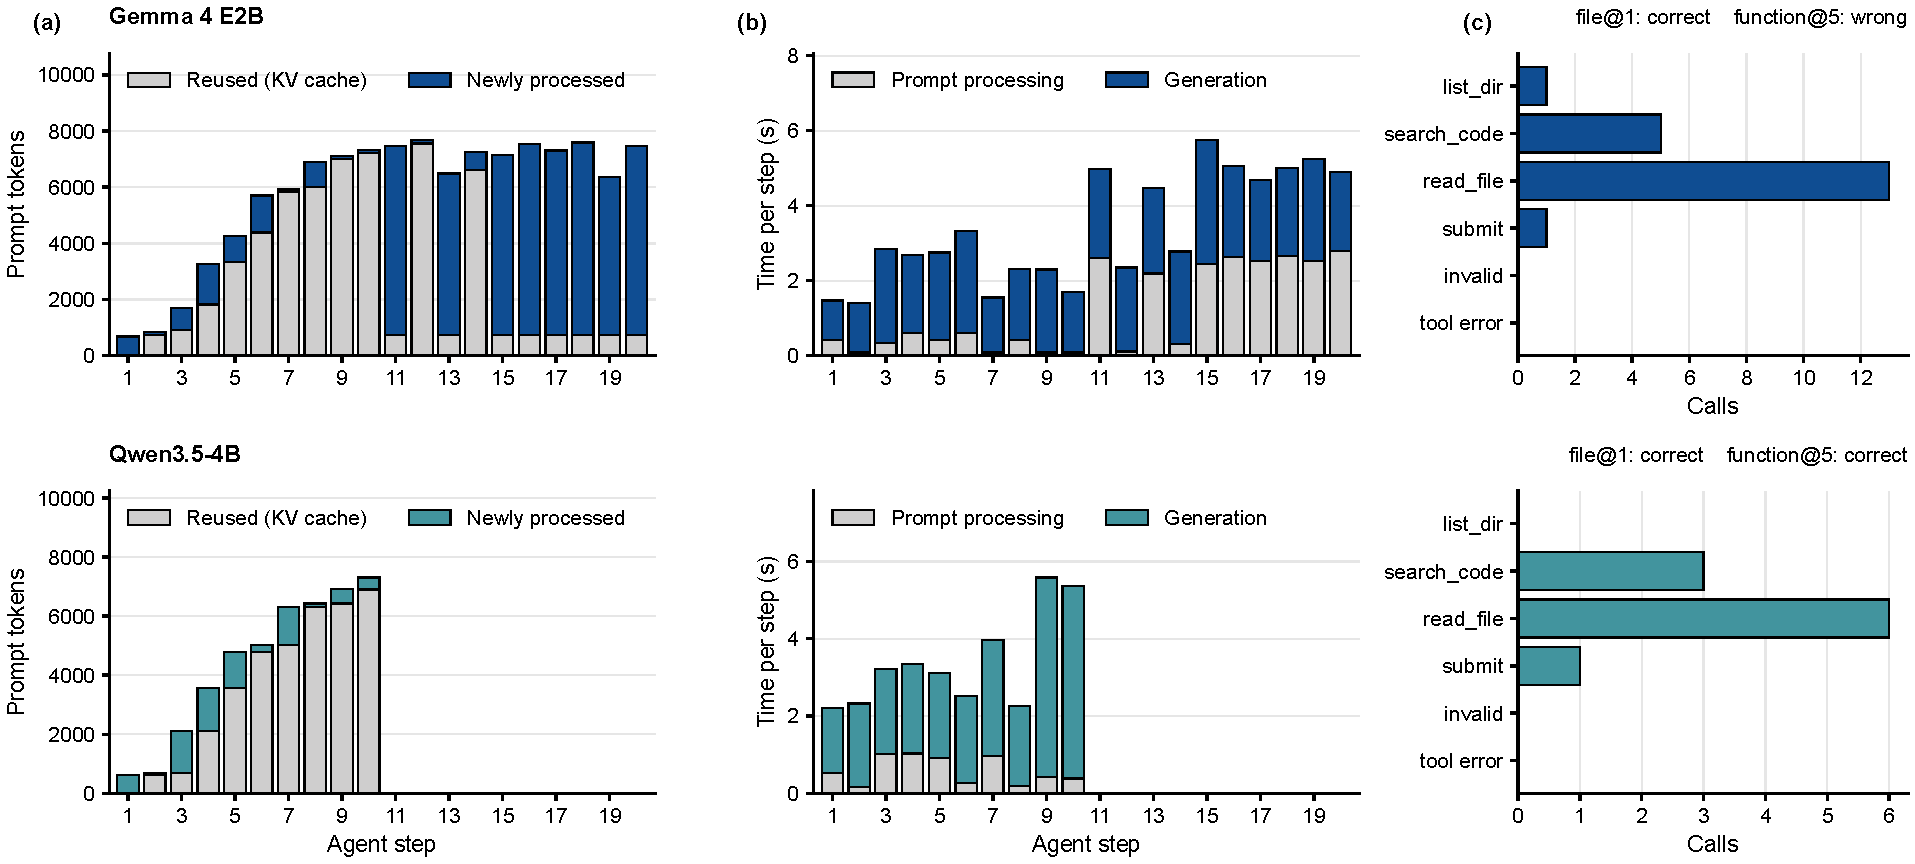
\includegraphics[width=\textwidth]{2026-10-25_02_e2e-smoke/figures/episode_astropy__astropy-12907.pdf}
\caption{\textbf{One episode per model} (task \texttt{astropy-12907}, configuration C1). (a)~Prompt tokens per step, split into reused (KV cache) and newly processed; once history compression starts (step 11 for \Gm{}), the cache is lost. (b)~Time per step. (c)~Tool calls. \Gm{} uses all 20 steps and names a wrong function; \Qw{} answers correctly in 10.}
\label{fig:smoke}
\end{figure}

\subsection{Answer format: form versus content}
\label{sec:dev-format}
With C1, both models reach 83\% \fileone{}, but function accuracy is 20--40 points lower, and 43\% of \Qw{}'s answers write functions in a module style (\texttt{pydicom.dataset.Dataset.to\_json\_dict}) instead of the requested \texttt{path.py::Name}.
Forcing the requested format with a regex in the grammar (experiment 04) removed every malformed name, yet halved \Qw{}'s \funcfive{} from 62\% to 33\% (6 tasks lost, none gained, $p=0.031$, the only significant change on the dev split).
The model begins its preferred dotted form, and the grammar does not let the string end without \texttt{.py::}, so the model fills it with junk until the length bound forces the suffix:
\begin{center}
\small\texttt{pvlib.iam.physical.physical\_1\_interface\_2\_interface\_3\_interface\_..\_.py::physical}
\end{center}
A \emph{structured} format, which gives the file and the name separate fields, recovers these answers (\Qw{} \funcfive{} 76\%), but hurts \Gm{} (43\%\,$\to$\,29\%), which leaves the function list empty in two tasks.
The repeated-call guard and budget hints then cut \Gm{}'s forced submissions from 57\% to 9\% without changing accuracy, and ranked lists let \Gm{}'s second and third guesses count (\funcfive{} 33\%\,$\to$\,43\%).
Figure~\ref{fig:devablation} shows the ladder.

\begin{figure}[t]
\centering
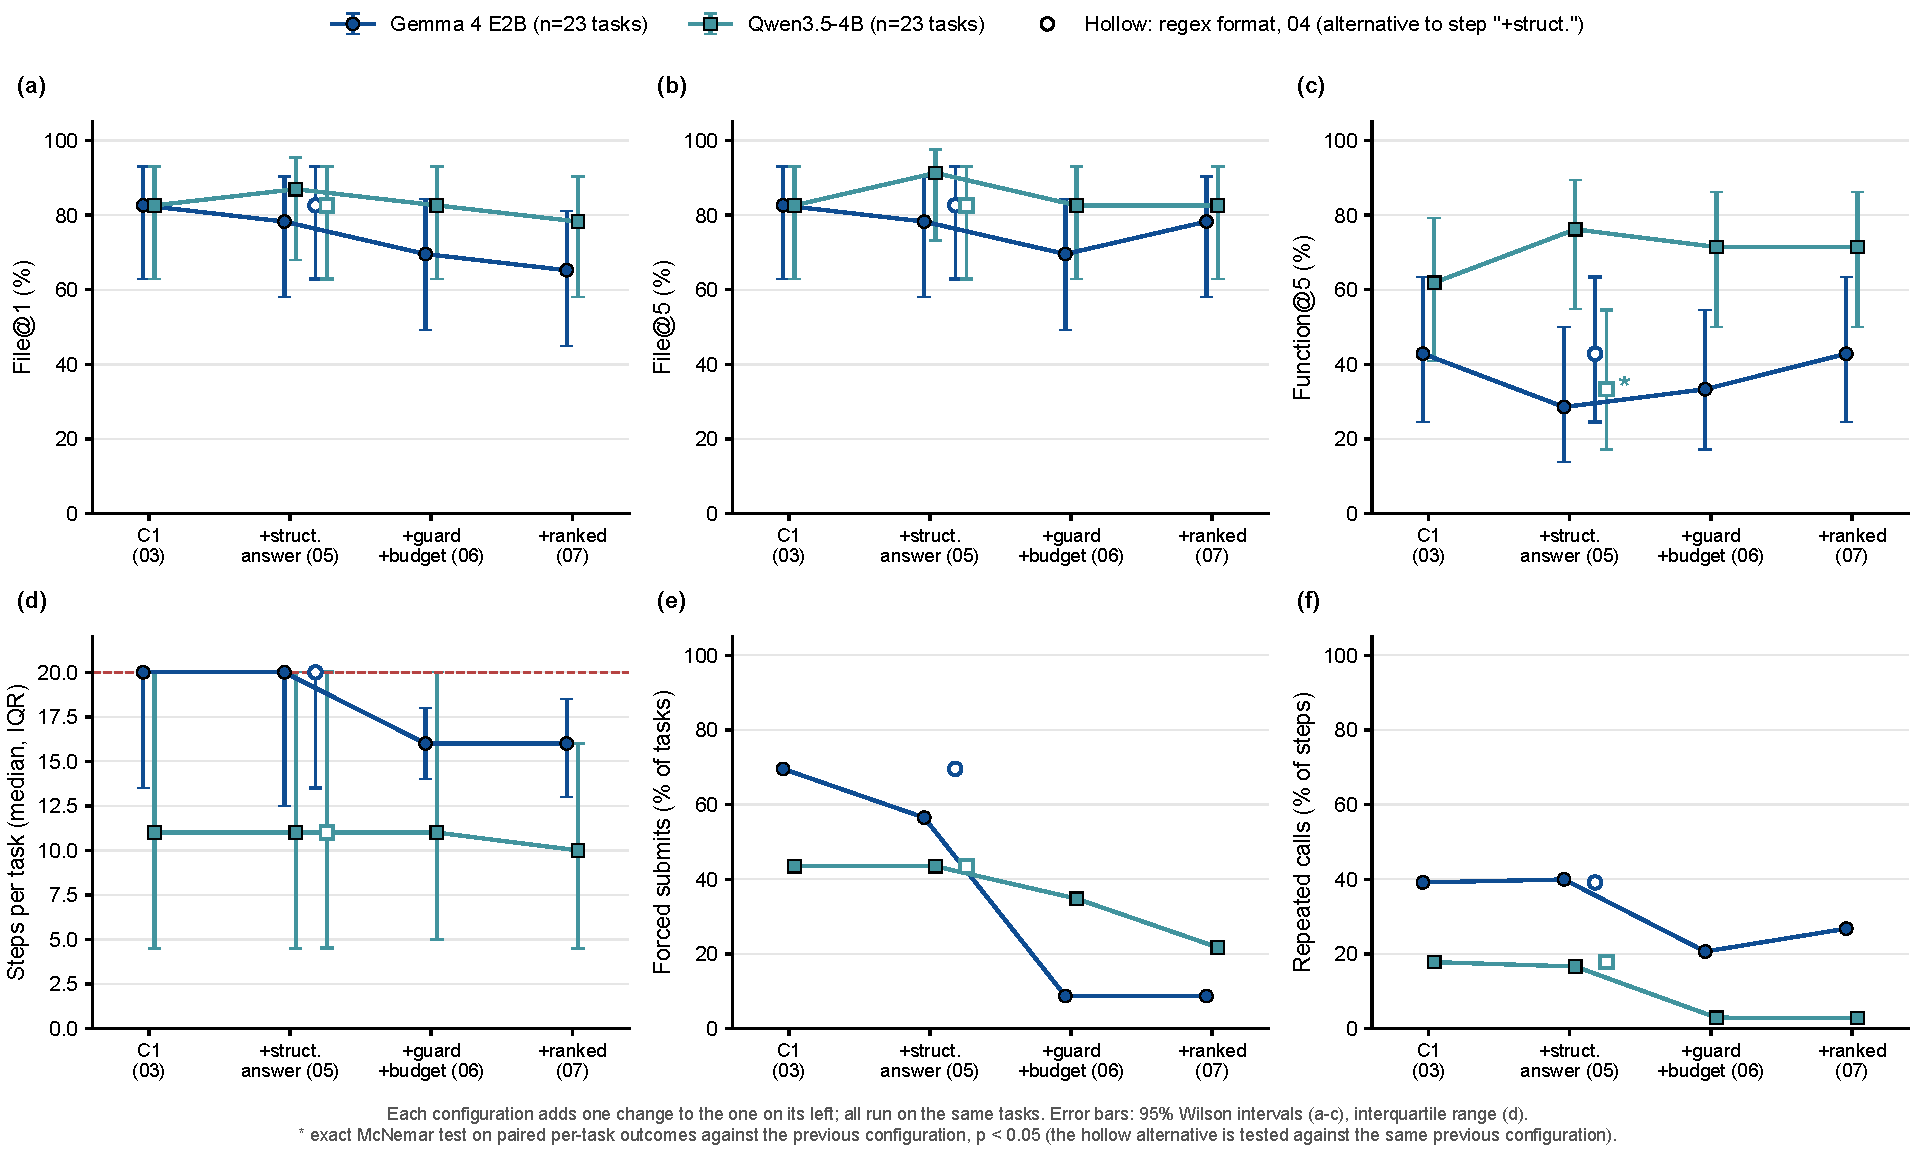
\includegraphics[width=\textwidth]{2026-10-25_08_dev-ablation/figures/ablation.pdf}
\caption{\textbf{Dev-split ablation ladder} (23 tasks; 21 with gold functions). Each step adds one change; the hollow marker is the regex-format alternative (experiment 04). Error bars: 95\% Wilson intervals; $*$: exact McNemar $p<0.05$ against the previous step.}
\label{fig:devablation}
\end{figure}

\begin{table}[t]
\centering
\small
\caption{\textbf{Dev split} (23 tasks, 6 repositories; \funcfive{} over 21 tasks). Percentages; experiment numbers refer to the result folders in the repository. C3$-$G (dev only) is C3 without grammar.}
\label{tab:dev}
\begin{tabular}{llccccccc}
\toprule
& & \multicolumn{3}{c}{\textcolor{gemma}{\Gm{}}} & \multicolumn{3}{c}{\textcolor{qwen}{\Qw{}}} \\
\cmidrule(lr){3-5}\cmidrule(lr){6-8}
Exp. & Configuration & File@1 & File@5 & Func@5 & File@1 & File@5 & Func@5 \\
\midrule
09 & C0: BM25 & 35 & 57 & 43 & 35 & 57 & 43 \\
03 & C1: file tools & 83 & 83 & 43 & 83 & 83 & 62 \\
04 & \quad + regex-forced names & 83 & 83 & 43 & 83 & 83 & \textbf{33} \\
05 & \quad + structured answers & 78 & 78 & 29 & 87 & 91 & \textbf{76} \\
06 & \quad + repeat guard, budget hints & 70 & 70 & 33 & 83 & 83 & 71 \\
07 & \quad + ranked lists (= C1+H) & 65 & 78 & 43 & 78 & 83 & 71 \\
10 & C2: + graph tools & 74 & 83 & 52 & 78 & 87 & 71 \\
11 & C3: + Evidence Buffer & 78 & 83 & 43 & 78 & 87 & 67 \\
12 & C3$-$G: C3 without grammar & 70 & 74 & 38 & 57 & 61 & 57 \\
\bottomrule
\end{tabular}
\end{table}

\paragraph{Graph tools and Evidence Buffer on dev.}
Graph tools gave \Gm{} its best dev accuracy (\funcfive{} 52\%) and left \Qw{} unchanged, but neither change was significant ($p\ge0.63$), and fewer than 10\% of calls went to the new tools.
The Evidence Buffer gave no gain and cost 43--52\% more time per task.
We therefore fixed C2 as the full system, kept C3 as an ablation row, and ran all configurations on the test set.

% ======================================================================
\section{Test-set results}
\label{sec:test}

Table~\ref{tab:main} gives the main results on the 100 test tasks, and Figure~\ref{fig:ablation} the ablation ladder with paired tests.

\begin{table}[t]
\centering
\caption{\textbf{Main results on the SWE-bench Lite test subset} (100 tasks; \funcfive{} over 88). Percentages with 95\% Wilson intervals; last two columns: median wall time per task in seconds (\Gm{} / \Qw{}).}
\label{tab:main}
\resizebox{\textwidth}{!}{%
\begin{tabular}{llccccccrr}
\toprule
& & \multicolumn{3}{c}{\textcolor{gemma}{\textbf{\Gm{}}}} & \multicolumn{3}{c}{\textcolor{qwen}{\textbf{\Qw{}}}} & \multicolumn{2}{c}{Time (s)} \\
\cmidrule(lr){3-5}\cmidrule(lr){6-8}\cmidrule(lr){9-10}
ID & Configuration & File@1 & File@5 & Func@5 & File@1 & File@5 & Func@5 & G & Q \\
\midrule
\inputrows{tables/main_results.tex}
\bottomrule
\end{tabular}}
\end{table}

\begin{figure}[t]
\centering
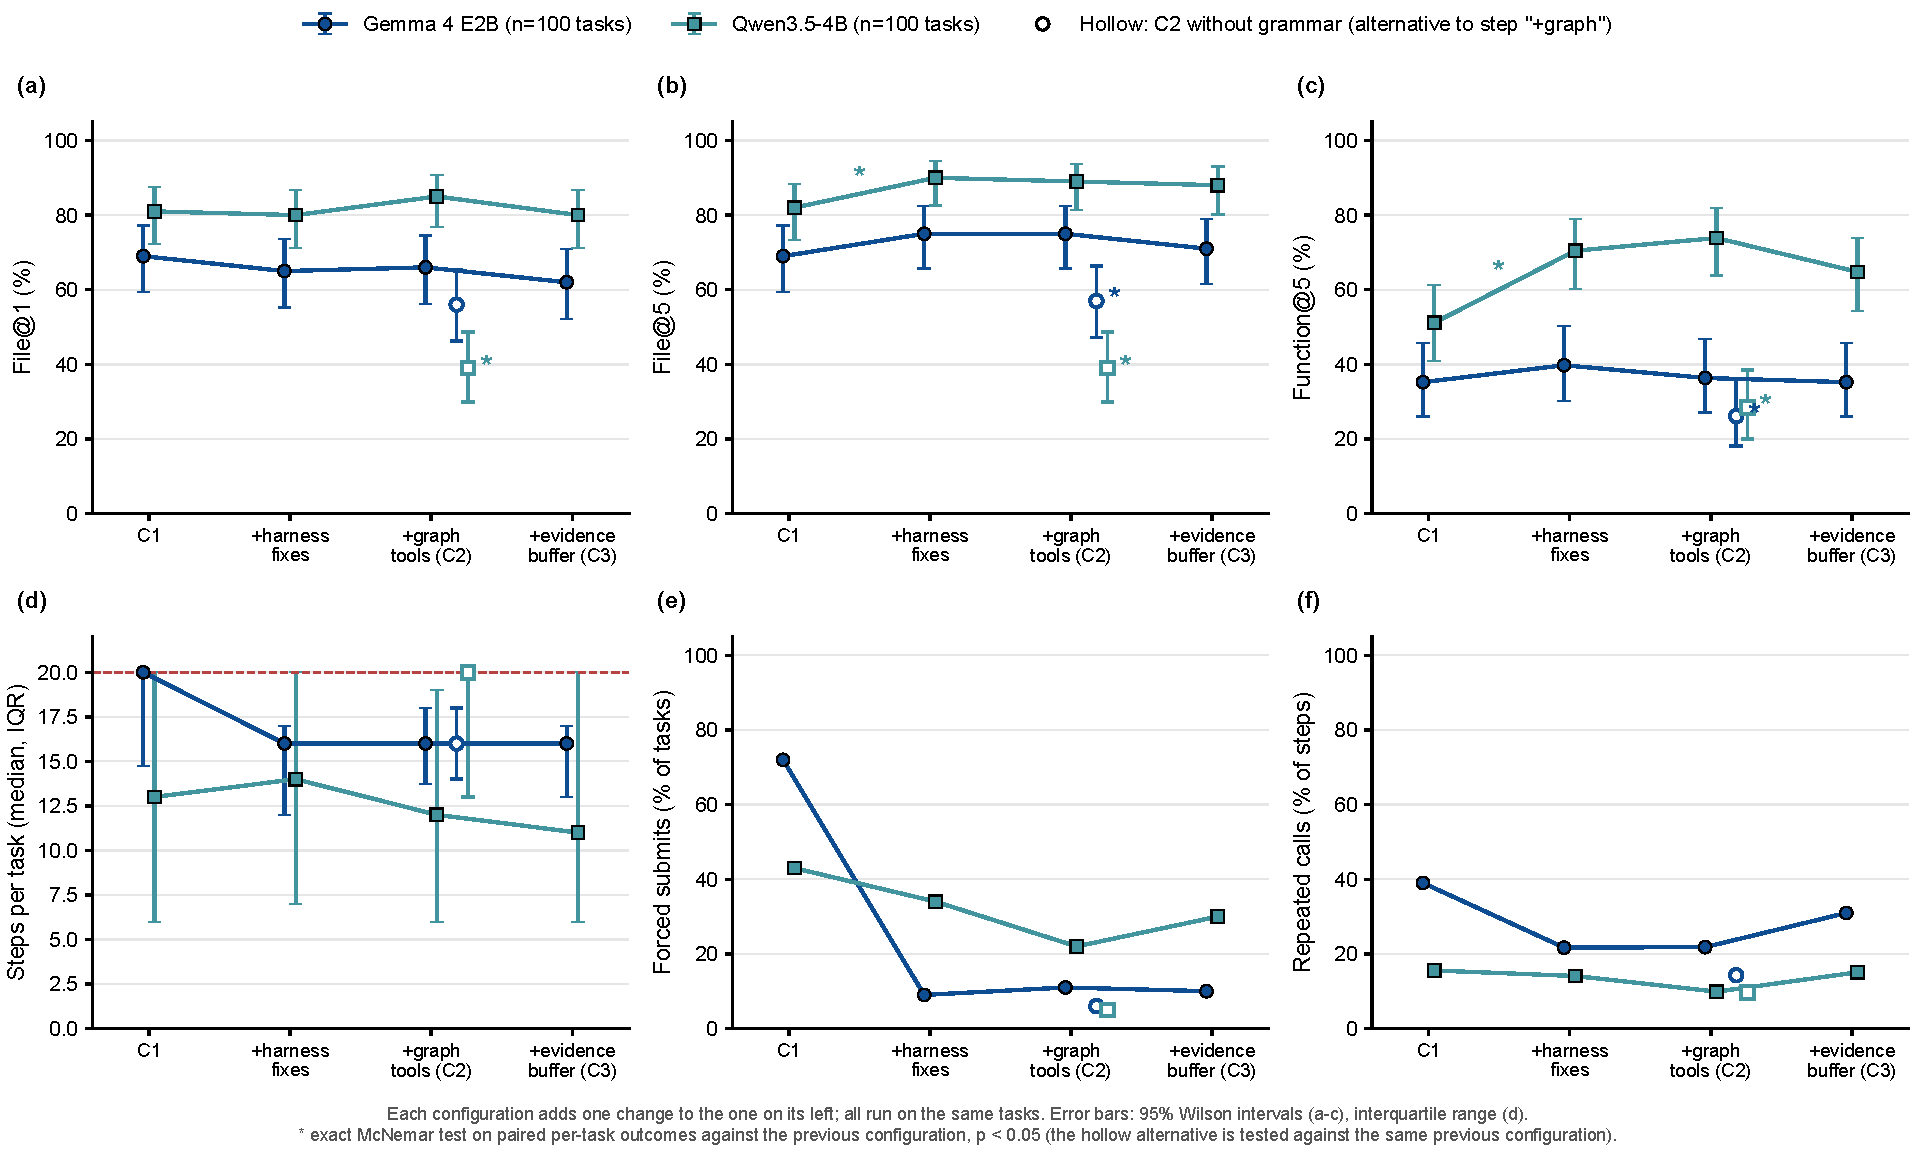
\includegraphics[width=\textwidth]{2026-11-10_19_test-ablation/figures/ablation.pdf}
\caption{\textbf{Test-set ablation ladder} (100 tasks; 88 with gold functions). (a--c)~Accuracy; (d)~steps per task (median, interquartile range; dashed line: 20-step limit); (e)~episodes that ended only because the last turn forced \texttt{submit}; (f)~share of steps repeating an earlier call. Hollow markers: C2 without grammar. Error bars: 95\% Wilson intervals; $*$: exact McNemar $p<0.05$ against the previous configuration (the hollow marker is tested against C1+H; the text compares it with C2).}
\label{fig:ablation}
\end{figure}

\subsection{Grammar-constrained decoding is essential (H2 supported)}
Compared with C2, removing the grammar drops \Qw{}'s \fileone{} from 85\% to 39\% (0 tasks gained, 46 lost, $p=3\times10^{-14}$) and its \funcfive{} from 74\% to 28\% (1 gained, 41 lost, $p=2\times10^{-11}$). \Gm{} loses 18 points of \filefive{} (1 gained, 19 lost, $p=4\times10^{-5}$); its drops in \fileone{} (66\%\,$\to$\,56\%, $p=0.052$) and \funcfive{} (36\%\,$\to$\,26\%, $p=0.11$) are not significant at $n=100$.
Figure~\ref{fig:grammar} breaks down why.
Free-text replies are invalid in 19\% (\Gm{}) and 23\% (\Qw{}) of steps, and at least one invalid reply occurs in 45\% and 79\% of episodes.
\Gm{}'s failures are all malformed JSON (unescaped characters, missing delimiters in long thoughts).
\Qw{}'s are mostly structural: in 173 steps it wrote a complete answer but omitted \texttt{"tool": "submit"}, putting the files directly into the action, and in 119 it named a tool that does not exist.
Because its final answer is the step it most often writes wrongly, 59\% of \Qw{}'s episodes end with an empty answer, against 0\% with the grammar.
A more forgiving parser would recover some of these answers, so the size of the drop depends partly on our parser; the grammar removes the need for such repair altogether.
The episodes also become longer: with the grammar, \Qw{} finishes half of its episodes within 12 steps, without it most run to the limit (Figure~\ref{fig:grammar}c).

\begin{figure}[t]
\centering
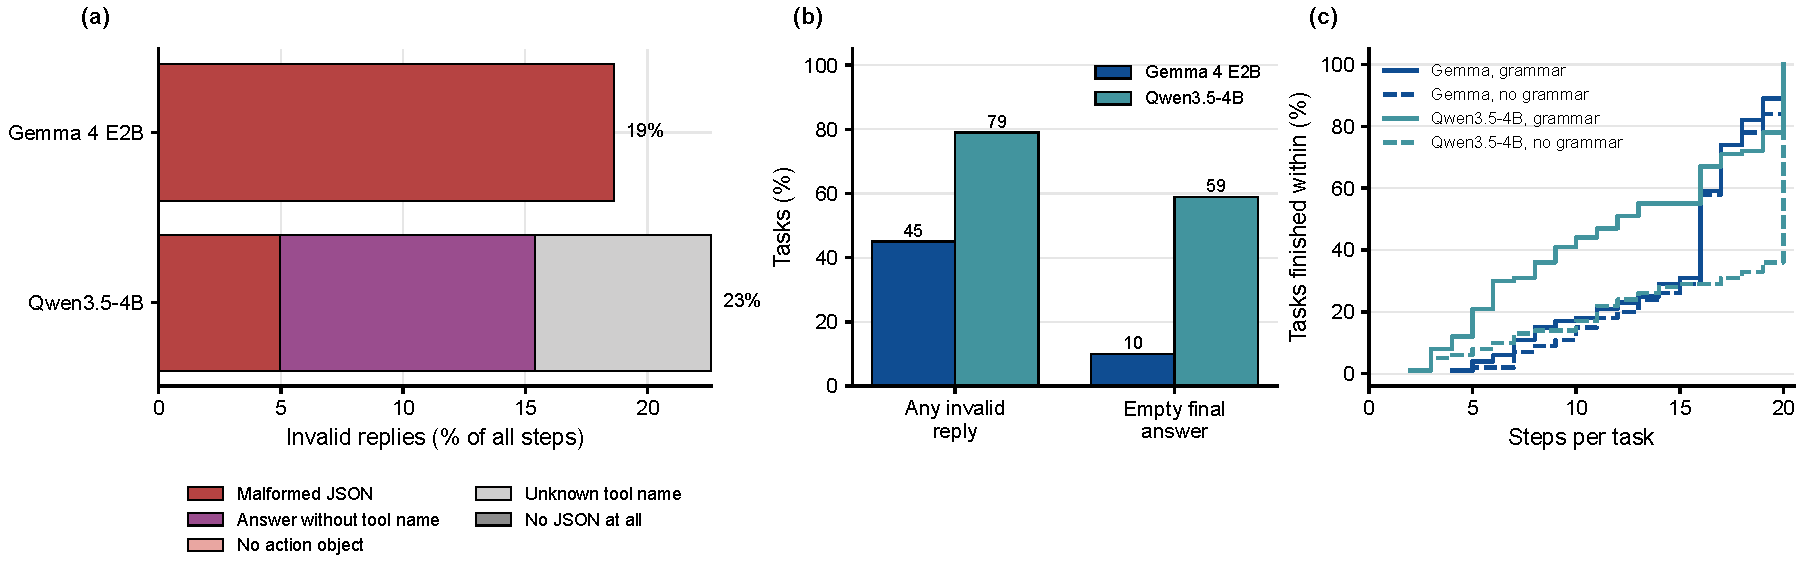
\includegraphics[width=\textwidth]{grammar_failures.pdf}
\caption{\textbf{What goes wrong without grammar-constrained decoding} (C2$-$G, 100 tasks). (a)~Invalid replies as a share of all steps, by type; ``answer without tool name'' is a well-formed final answer missing \texttt{"tool": "submit"}. (b)~Episodes with at least one invalid reply and with an empty final answer. (c)~Cumulative distribution of episode length with (solid) and without (dashed) the grammar.}
\label{fig:grammar}
\end{figure}

\subsection{Harness fixes help \Qw{}; graph tools and the Evidence Buffer do not (H1 mostly rejected)}
\paragraph{Harness fixes.} C1$\to$C1+H raises \Qw{}'s \funcfive{} from 51\% to 70\% (17 tasks gained, \emph{none} lost, $p=1.5\times10^{-5}$) and \filefive{} from 82\% to 90\% ($p=0.039$).
Malformed function names fall from 44\% of \Qw{}'s tasks to 1\%: the structured answer converts the model's existing knowledge into scorable answers.
For \Gm{}, the same fixes change behaviour (forced submissions 72\%\,$\to$\,9\%, repeated calls 39\%\,$\to$\,22\% of steps, mean time per task 51\,s\,$\to$\,40\,s) but none of its accuracy changes is significant.
\paragraph{Graph tools.} C1+H$\to$C2 changes no metric significantly for either model (\Qw{} \fileone{} +5 tasks, 0 lost, $p=0.063$).
Figure~\ref{fig:tools} shows why the effect is small: graph tools receive 11\% of \Gm{}'s and 9\% of \Qw{}'s calls, almost all of them \texttt{find\_definition}; in C2, \Qw{} calls \texttt{get\_code\_neighbors} and \texttt{get\_file\_outline} once each and never calls \texttt{search\_similar\_code}.
Both models keep spending most turns on \texttt{search\_code} and \texttt{read\_file}.
\paragraph{Evidence Buffer.} C2$\to$C3 lowers every accuracy metric for both models (none significantly; \Qw{} \funcfive{} 74\%\,$\to$\,65\%, 5 gained, 13 lost, $p=0.096$), while generating 27\% (\Gm{}) and 17\% (\Qw{}) more tokens and taking 23\% and 14\% longer per task (Figure~\ref{fig:cost}).
Within a 20-turn, ${\sim}$6K-token history, little context is lost, so the buffer pays its cost without a problem to solve.

\begin{figure}[t]
\centering
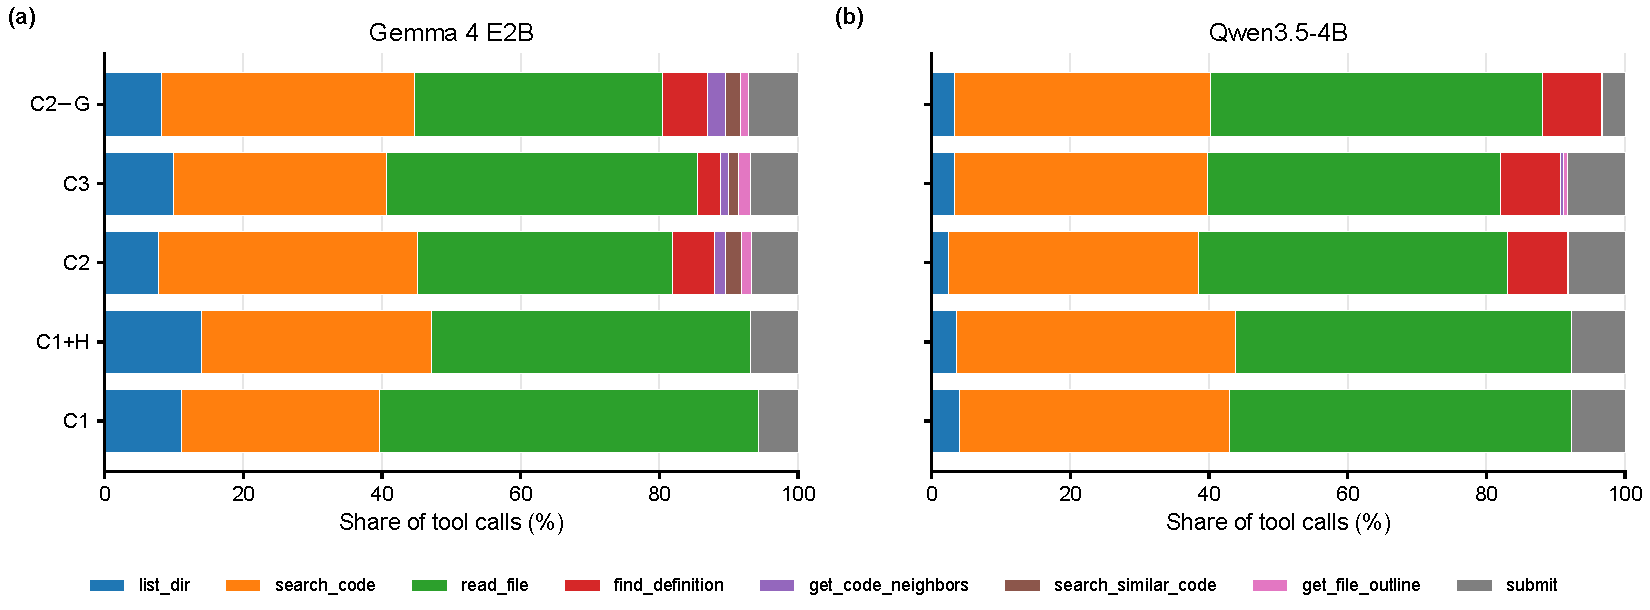
\includegraphics[width=\textwidth]{tool_usage.pdf}
\caption{\textbf{Tool usage by configuration} (share of all tool calls, 100 tasks). Graph tools (red, purple, brown, pink) are available from C2 on but receive about one call in ten; \texttt{find\_definition} accounts for most of them.}
\label{fig:tools}
\end{figure}

\begin{figure}[t]
\centering
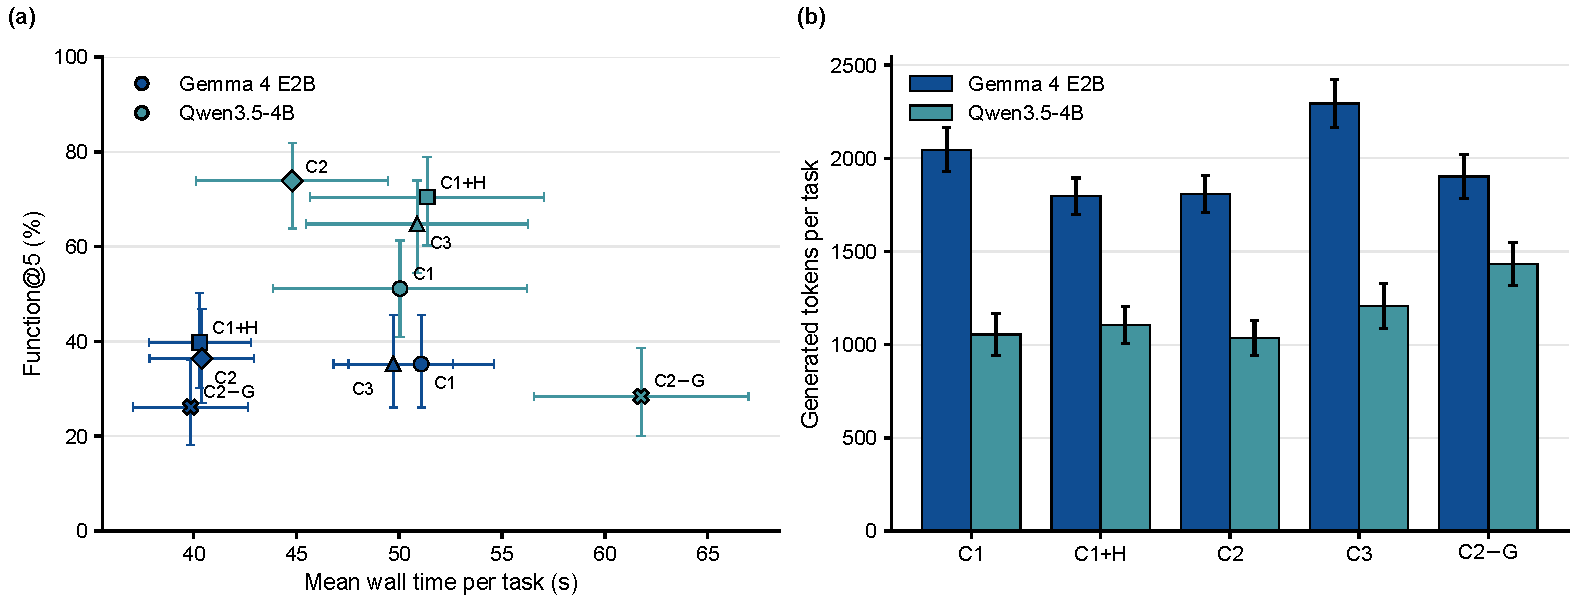
\includegraphics[width=\textwidth]{cost_accuracy.pdf}
\caption{\textbf{Cost and accuracy.} (a)~\funcfive{} against mean wall time per task (error bars: 95\% Wilson interval and 95\% CI of the mean). (b)~Generated tokens per task (mean, 95\% CI). On a 4\,GB GPU, generation dominates time, so components that make the model write more (Evidence Buffer, free-text replies) are expensive.}
\label{fig:cost}
\end{figure}

\subsection{Model families differ (H3 partly supported)}
\Qw{} is the stronger localizer in every configuration (Table~\ref{tab:main}), by 12--19 points of \fileone{} and 16--38 points of \funcfive{} with the grammar on.
The two models also respond differently to the same change: the structured answer format and ranked lists lift \Qw{} and do little for \Gm{}, and on the dev split the structured format hurt \Gm{}.
What does transfer across families is the effect of the grammar, and the absence of a gain from graph tools and the Evidence Buffer.

\subsection{Comparison with retrieval}
BM25 (C0) reaches 33\% \fileone{}, 64\% \filefive{} and 36\% \funcfive{} (47\% at Function@10) in about 2\,s per task on the CPU.
The agents' advantage is concentrated in the top file: \Gm{} C2 gains 41 tasks of \fileone{} over BM25 and loses 8 ($p=2\times10^{-6}$), \Qw{} gains 55 and loses 3.
At function level, \Qw{} C2 beats BM25 clearly (74\% vs.\ 36\%, 37 gained, 4 lost, $p=10^{-7}$), but \Gm{} C2 ties it (36\% vs.\ 36\%, 14 gained, 14 lost).
Figure~\ref{fig:repos} shows the same pattern per repository: the agents dominate BM25 on file localization almost everywhere, while \Gm{}'s function-level accuracy stays near BM25's on the two largest repositories (django, sympy).

\begin{figure}[t]
\centering
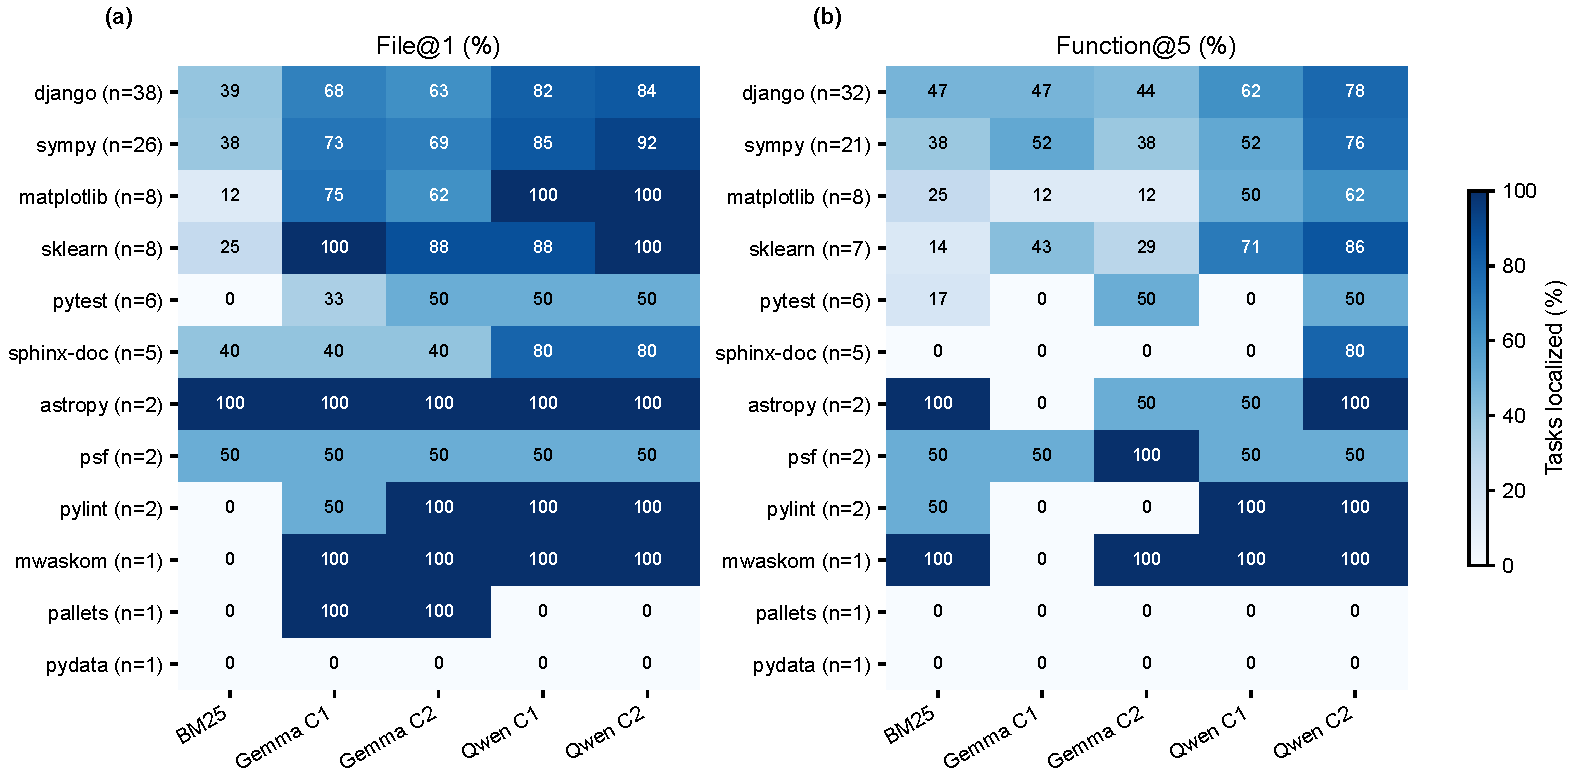
\includegraphics[width=0.95\textwidth]{repo_heatmap.pdf}
\caption{\textbf{Accuracy per repository} on the test subset ($n$ = tasks per repository; function metrics exclude tasks without gold functions). Repositories with one or two tasks are shown for completeness, not for comparison.}
\label{fig:repos}
\end{figure}

\subsection{Ranked lists, complementarity and headroom}
Ranked lists add real but modest value: when the correct file is not first, it is second or third in 9--10\% of tasks for \Gm{} and 4--10\% for \Qw{} (Figure~\ref{fig:rank}).
Both models submit exactly the minimum of three candidates, so the lists act as a floor rather than as calibrated rankings.

The two models' successes are nearly nested (Figure~\ref{fig:overlap}a): among 88 tasks, \Qw{} C2 solves 37 that \Gm{} C2 misses, while \Gm{} solves only 4 that \Qw{} misses; 19 tasks defeat both.
Across configurations, however, there is headroom: a task is solved by \emph{some} configuration of \Gm{} in 62\% of cases (best single configuration: 40\%) and of \Qw{} in 82\% (best: 74\%); any configuration of either model covers 85\%, and adding BM25 only reaches 86\% (Figure~\ref{fig:overlap}b).
Greedy decoding is deterministic, so this spread comes from the configurations, not from sampling: small changes to the prompt or tools change which tasks succeed, which suggests that ensembling or self-consistency across configurations could close part of the gap.

\begin{figure}[t]
\centering
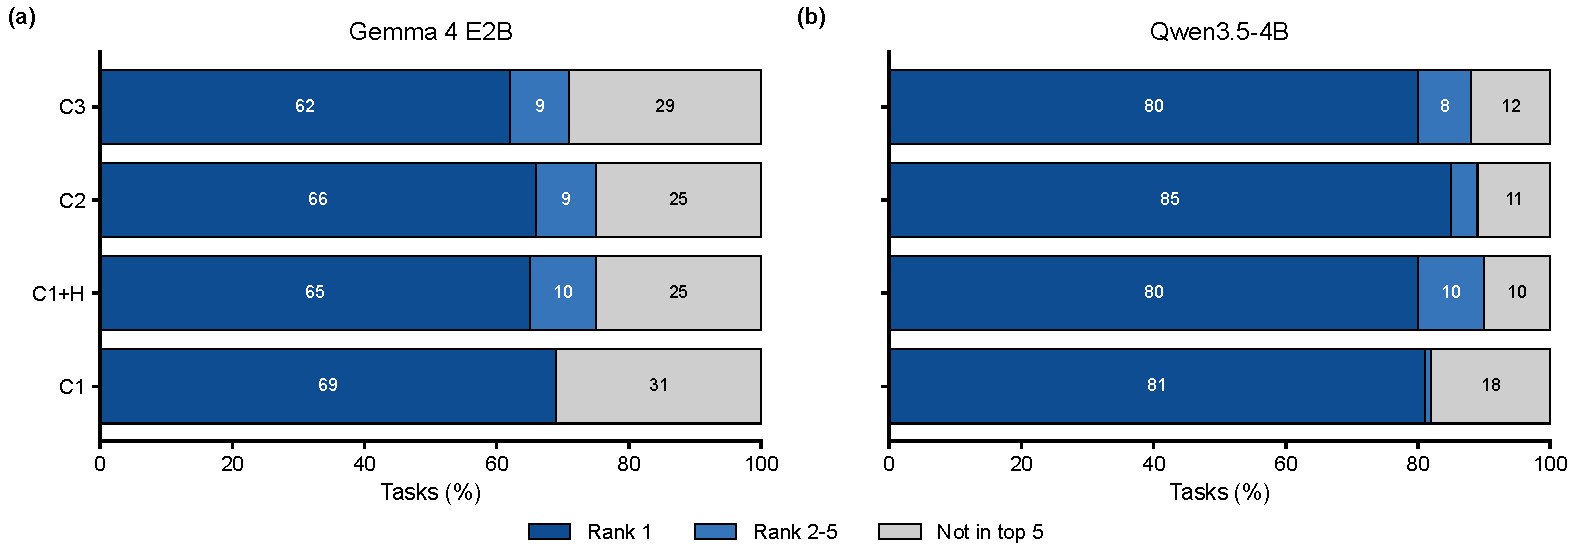
\includegraphics[width=0.9\textwidth]{file_rank.pdf}
\caption{\textbf{Rank of the first correct file} in the submitted list. C1 asks for up to five files but the models submit about one; from C1+H on, at least three are required. No model ever submits more than three files, so ranks 4--5 are empty.}
\label{fig:rank}
\end{figure}

\begin{figure}[t]
\centering
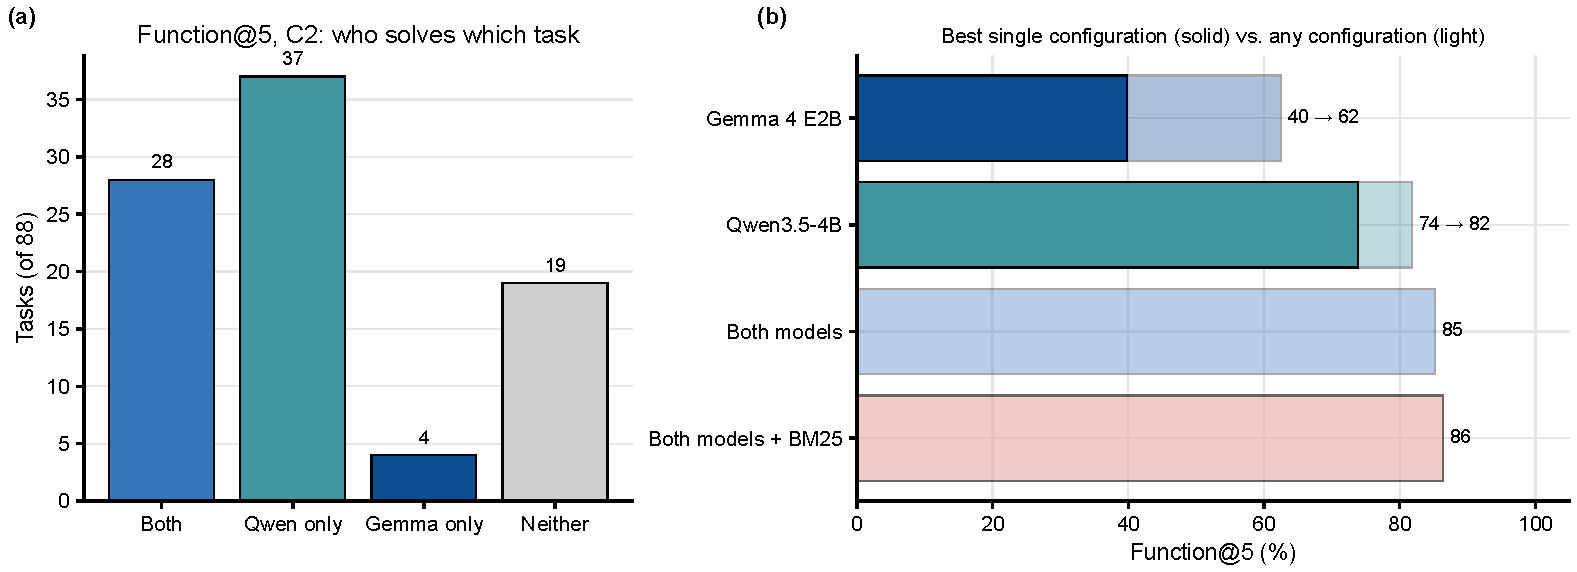
\includegraphics[width=\textwidth]{overlap_oracle.pdf}
\caption{\textbf{Complementarity and headroom} (\funcfive{}, 88 tasks). (a)~Which model solves which task with configuration C2. (b)~Best single configuration (solid) against the share of tasks solved by at least one configuration (light), per model, for both models together, and with BM25 added.}
\label{fig:overlap}
\end{figure}

\subsection{Does the dev split predict the test split?}
Figure~\ref{fig:devtest} compares the same configurations on both splits.
For \Qw{} the dev split is a good guide (all \funcfive{} points within 11 points of the diagonal).
For \Gm{} it is optimistic: \fileone{} drops by 8--16 points from dev to test in three of four configurations, and C2's dev advantage (\funcfive{} 52\%) disappears on the test set (36\%), which is consistent with the wide dev intervals ($n=21$).
With 23 tasks, only changes of about six tasks in one direction are detectable; dev results should guide engineering, not support claims.

\begin{figure}[t]
\centering
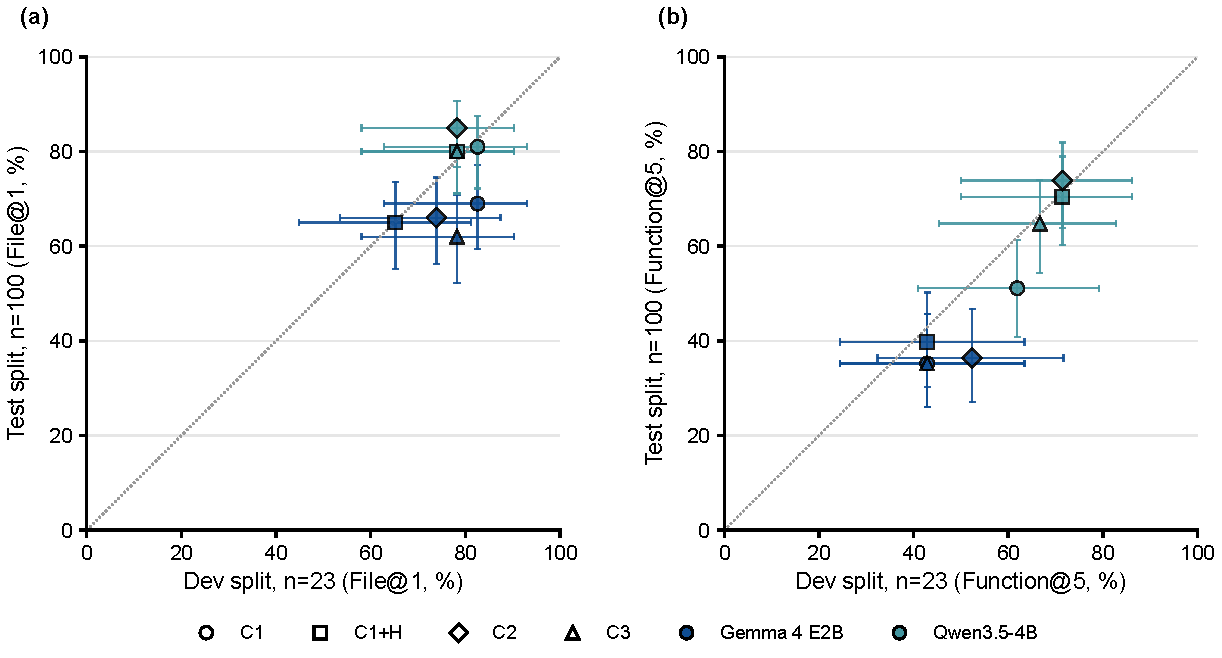
\includegraphics[width=0.8\textwidth]{dev_vs_test.pdf}
\caption{\textbf{Dev versus test accuracy} for the same configurations (error bars: 95\% Wilson intervals; dotted: equality). Dev results overestimate \Gm{}'s test accuracy.}
\label{fig:devtest}
\end{figure}

% ======================================================================
\section{Discussion}
\label{sec:discussion}

\paragraph{Control the output, not the search.}
The components that helped are those that control what the model emits: the grammar that makes every turn a valid call, the structured answer that separates file from function, and the guards that make the model stop.
The components that extend the search (graph tools, an evidence memory) did not help, and the tool-usage data explain why: small models largely ignore tools they were not trained to rely on and fall back to grep-and-read.
Tool \emph{availability} is not tool \emph{adoption}.
For small models, graph information may have to be pushed into the prompt (for example, showing definitions of identifiers that appear in the issue) instead of offered as a tool to pull.

\paragraph{Constraints must follow the model.}
The regex experiment and the free-text failures are two sides of the same issue.
Unconstrained, \Qw{} writes sensible answers in a slightly wrong shape; constrained in a way that disagrees with its preferred shape, it writes junk to satisfy the constraint.
A constraint works when it leaves room for what the model is already trying to write (separate fields, permissive names), and fails when it forces a token sequence the model has not planned.

\paragraph{Behaviour fixes are not accuracy fixes.}
\Gm{}'s looping (72\% forced submissions in C1) looked like the cause of its errors, but stopping it saved 21\% of time and changed accuracy by nothing measurable: it looped because it did not know where to look.
Behavioural metrics are useful for cost but are poor proxies for accuracy.

\paragraph{Hypotheses.}
H1 is supported only for the harness fixes, and only for \Qw{}; graph tools and the Evidence Buffer do not help.
H2 is supported for both small models; we could not test whether the grammar matters less for large models (Section~\ref{sec:future}).
H3 is partly supported: the grammar effect transfers across families, the effect of answer-format changes does not.
H4 was not tested: the repair experiment was not run within this study.

% ======================================================================
\section{Limitations}
\label{sec:limitations}
\begin{itemize}
\item \textbf{Sample size.} 100 test tasks (88 with gold functions) detect differences of roughly 10--15 points between paired configurations; smaller effects, such as those of graph tools, remain unresolved. The dev split has only 23 tasks.
\item \textbf{One run per configuration.} Decoding is greedy with a fixed seed, so runs are deterministic, but results may be sensitive to prompt wording, which we did not vary systematically.
\item \textbf{Two models, one quantization each.} Results may differ for other families (e.g., Phi, Llama) and for higher-precision weights.
\item \textbf{Parser dependence.} The C2$-$G drop includes failures a more forgiving parser could repair (Section~\ref{sec:test}); it measures our harness without the grammar, not the best possible free-text harness.
\item \textbf{Gold locations.} Gold functions are derived from the reference patch; other valid fixes may edit different functions. All gold patches in the subset touch one file.
\item \textbf{No large-model reference and no repair experiment} (Section~\ref{sec:future}).
\end{itemize}

% ======================================================================
\section{Future work}
\label{sec:future}
\begin{itemize}
\item \textbf{Large-model reference.} We planned to run C2 with Gemma~4 31B through the free Gemini API on 50 test tasks (about 600--750 requests), to test whether the grammar and harness matter less at scale (H2). Under the free-tier request limits available to us, the run would have taken roughly a week of continuous scheduling, so it is left for future work.
\item \textbf{Repair (H4).} Run the best configuration end to end, generating and testing patches on a subset, to measure how far a 4\,GB GPU gets on fixing.
\item \textbf{Ensembles over configurations.} The 85\% union across configurations (Figure~\ref{fig:overlap}) suggests voting or self-consistency across prompts and tool sets.
\item \textbf{Pushed graph context.} Inject graph lookups automatically instead of exposing them as tools.
\item \textbf{Scale.} The full 300-task test split, a third model family, and longer budgets, where an Evidence Buffer may start to pay off.
\end{itemize}

% ======================================================================
\section{Conclusion}
Off-the-shelf models of 2--4B parameters, running offline on a 4\,GB laptop GPU without training, can localize the right file for 85\% and the right function for 74\% of SWE-bench Lite test issues in under a minute each, with the right scaffolding.
The right scaffolding, however, is not the search-heavy design that works for large models.
It is the part that controls the output: grammar-constrained decoding, an answer format that matches how the model already writes, and simple guards.
For small models, getting the answer out matters as much as finding it.

\paragraph{Reproducibility.}
The repository contains the harness (\texttt{agent/}), run scripts (\texttt{scripts/}), every experiment's configuration, per-task results and figures (\texttt{results/}), and the code that regenerates every figure and table in this paper from those results (\texttt{analysis/}, \texttt{paper/}). Full trajectories are kept outside the repository because of their size.

% ======================================================================
\begin{thebibliography}{99}\small
\bibitem[Chen et~al.(2025)]{chen2025locagent}
Z.~Chen, X.~Tang, G.~Deng, F.~Wu, J.~Wu, Z.~Jiang, V.~Prasanna, A.~Cohan, and X.~Wang.
\newblock {LocAgent}: Graph-guided {LLM} agents for code localization.
\newblock In \emph{Proceedings of ACL}, 2025.
\newblock arXiv:2503.09089.

\bibitem[Geng et~al.(2023)]{geng2023grammar}
S.~Geng, M.~Josifoski, M.~Peyrard, and R.~West.
\newblock Grammar-constrained decoding for structured {NLP} tasks without finetuning.
\newblock In \emph{Proceedings of EMNLP}, 2023.
\newblock arXiv:2305.13971.

\bibitem[Jimenez et~al.(2024)]{jimenez2024swebench}
C.~E. Jimenez, J.~Yang, A.~Wettig, S.~Yao, K.~Pei, O.~Press, and K.~Narasimhan.
\newblock {SWE-bench}: Can language models resolve real-world {GitHub} issues?
\newblock In \emph{Proceedings of ICLR}, 2024.
\newblock arXiv:2310.06770.

\bibitem[Robertson and Zaragoza(2009)]{robertson2009bm25}
S.~Robertson and H.~Zaragoza.
\newblock The probabilistic relevance framework: {BM25} and beyond.
\newblock \emph{Foundations and Trends in Information Retrieval}, 3(4):333--389, 2009.

\bibitem[Tam et~al.(2024)]{tam2024speak}
Z.~R. Tam, C.-K. Wu, Y.-L. Tsai, C.-Y. Lin, H.-y. Lee, and Y.-N. Chen.
\newblock Let me speak freely? {A} study on the impact of format restrictions on performance of large language models.
\newblock In \emph{Proceedings of EMNLP: Industry Track}, 2024.
\newblock arXiv:2408.02442.

\bibitem[Willard and Louf(2023)]{willard2023outlines}
B.~T. Willard and R.~Louf.
\newblock Efficient guided generation for large language models.
\newblock arXiv:2307.09702, 2023.

\bibitem[Xia et~al.(2024)]{xia2024agentless}
C.~S. Xia, Y.~Deng, S.~Dunn, and L.~Zhang.
\newblock Agentless: Demystifying {LLM}-based software engineering agents.
\newblock arXiv:2407.01489, 2024.

\bibitem[Yang et~al.(2024)]{yang2024sweagent}
J.~Yang, C.~E. Jimenez, A.~Wettig, K.~Lieret, S.~Yao, K.~Narasimhan, and O.~Press.
\newblock {SWE-agent}: Agent-computer interfaces enable automated software engineering.
\newblock In \emph{Advances in NeurIPS}, 2024.
\newblock arXiv:2405.15793.

\bibitem[Yao et~al.(2023)]{yao2023react}
S.~Yao, J.~Zhao, D.~Yu, N.~Du, I.~Shafran, K.~Narasimhan, and Y.~Cao.
\newblock {ReAct}: Synergizing reasoning and acting in language models.
\newblock In \emph{Proceedings of ICLR}, 2023.
\newblock arXiv:2210.03629.

\bibitem[Zhang et~al.(2024)]{zhang2024autocoderover}
Y.~Zhang, H.~Ruan, Z.~Fan, and A.~Roychoudhury.
\newblock {AutoCodeRover}: Autonomous program improvement.
\newblock In \emph{Proceedings of ISSTA}, 2024.
\newblock arXiv:2404.05427.
\end{thebibliography}

% ======================================================================
\clearpage
\appendix
\section{Run details}
\label{app:details}

\begin{table}[H]
\centering
\small
\caption{Run parameters shared by all agent configurations.}
\begin{tabular}{ll}
\toprule
Parameter & Value \\
\midrule
Runtime & llama.cpp \texttt{llama-server} b11873, CUDA, all layers on GPU, flash attention \\
Models & \Gm{} (QAT Q4\_0, 3.1\,GB file); \Qw{} (Q4\_K\_M, 2.6\,GB file) \\
Context & 12{,}288 tokens, one slot, non-thinking mode \\
Decoding & greedy (temperature 0, seed 0); grammar from the reply JSON schema (except C2$-$G) \\
Episode & 20 turns; last turn allows only \texttt{submit} \\
Prompt budget & issue $\le$ 6{,}000 chars; tool output $\le$ 4{,}000 chars; history $\le$ 22{,}000 chars \\
Data & SWE-bench Lite dev (23 tasks) and a seeded, repository-stratified 100-task test subset \\
Compute & 1{,}000 test episodes, 13.3\,h total wall time on one RTX 2050 \\
\bottomrule
\end{tabular}
\end{table}

\paragraph{System prompt.}
\begin{quote}\small\ttfamily
You are a software engineer finding the location of a bug in a Python repository. Read the GitHub issue, explore the code with the tools, and submit the files and functions that must be edited to fix the issue. Do not write a fix.\\
Tools: \{tool descriptions\}\\
Reply with exactly one JSON object per turn: \{"thought": "<one or two sentences>", "action": \{"tool": "<tool name>", ...arguments\}\}\\
You have 20 turns. Submit as soon as you are confident.
\end{quote}

\paragraph{Experiment index.}
Every experiment lives in \texttt{results/<date>\_<NN>\_<name>/} with its configuration, per-task results, metrics, figures and (for dev experiments) notes:
01 hardware benchmark; 02 end-to-end smoke test; 03 C1 (dev); 04 regex function names (dev); 05 structured answers (dev); 06 repeat guard and budget hints (dev); 07 ranked lists (dev); 08 dev ablation; 09 C0 BM25 (dev); 10 C2 (dev); 11 C3 (dev); 12 C3$-$G (dev); 13 C0 (test); 14 C2 (test); 15 C1 (test); 16 C1+H (test); 17 C3 (test); 18 C2$-$G (test); 19 test ablation.

% ----------------------------------------------------------------------
\clearpage
\section{Per-experiment figures}
\label{app:figures}

Each experiment's summary figure shows (a)~accuracy with 95\% Wilson intervals, (b)~agent steps and (c)~wall time per task, (d)~failure modes and, from experiment 07 on, (e)~tool usage. The outcome figures mark, for every task, whether the model found the file only, the file and the function, or neither (top-5).

\newcommand{\expfig}[3]{%
\begin{figure}[H]\centering
\includegraphics[width=#3\textwidth]{#1}
\caption{#2}
\end{figure}}

\subsection{Development split}
\expfig{2026-10-25_03_c1-dev/figures/summary.pdf}{\textbf{Exp.\ 03, C1 on dev.} File tools only. Both models find the file in 83\% of tasks; function accuracy is lower, \Gm{} hits the step limit in 70\% of episodes, and 43\% of \Qw{}'s tasks contain malformed function names.}{0.92}
\expfig{2026-10-25_04_fmt-dev/figures/summary.pdf}{\textbf{Exp.\ 04, regex-forced function names (dev).} Malformed names vanish, but \Qw{}'s \funcfive{} falls from 62\% to 33\%: the regex corrupts answers the model was writing in its own format.}{0.92}
\expfig{2026-10-25_05_struct-dev/figures/summary.pdf}{\textbf{Exp.\ 05, structured answers (dev).} \Qw{} \funcfive{} rises to 76\%; \Gm{} falls to 29\%, leaving function lists empty in two tasks.}{0.92}
\expfig{2026-10-25_06_guard-dev/figures/summary.pdf}{\textbf{Exp.\ 06, repeat guard and budget hints (dev).} \Gm{}'s forced submissions fall from 57\% to 9\% and its time per task by 26\%, with no accuracy change.}{0.92}
\expfig{2026-10-25_07_ranked-dev/figures/summary.pdf}{\textbf{Exp.\ 07, ranked lists (dev).} Both models submit exactly three candidates; \Gm{}'s \funcfive{} rises to 43\%, top-1 accuracy drops slightly for both.}{0.92}
\expfig{2026-10-25_09_c0-dev/figures/summary.pdf}{\textbf{Exp.\ 09, C0 BM25 retrieval (dev).} 35\% \fileone{}, 43\% \funcfive{}, about 2\,s per task on the CPU.}{0.92}
\expfig{2026-10-25_10_c2-dev/figures/summary.pdf}{\textbf{Exp.\ 10, C2 graph tools (dev).} \Gm{} reaches its best dev accuracy (\funcfive{} 52\%); graph tools receive under 10\% of calls.}{0.92}
\expfig{2026-10-25_11_c3-dev/figures/summary.pdf}{\textbf{Exp.\ 11, C3 Evidence Buffer (dev).} No accuracy gain, 43--52\% more time per task.}{0.92}
\expfig{2026-10-26_12_c4g-dev/figures/summary.pdf}{\textbf{Exp.\ 12, C3 without grammar (dev).} Invalid replies appear in 39\% (\Gm{}) of episodes; \Qw{}'s \fileone{} falls to 57\%.}{0.92}

\begin{figure}[H]\centering
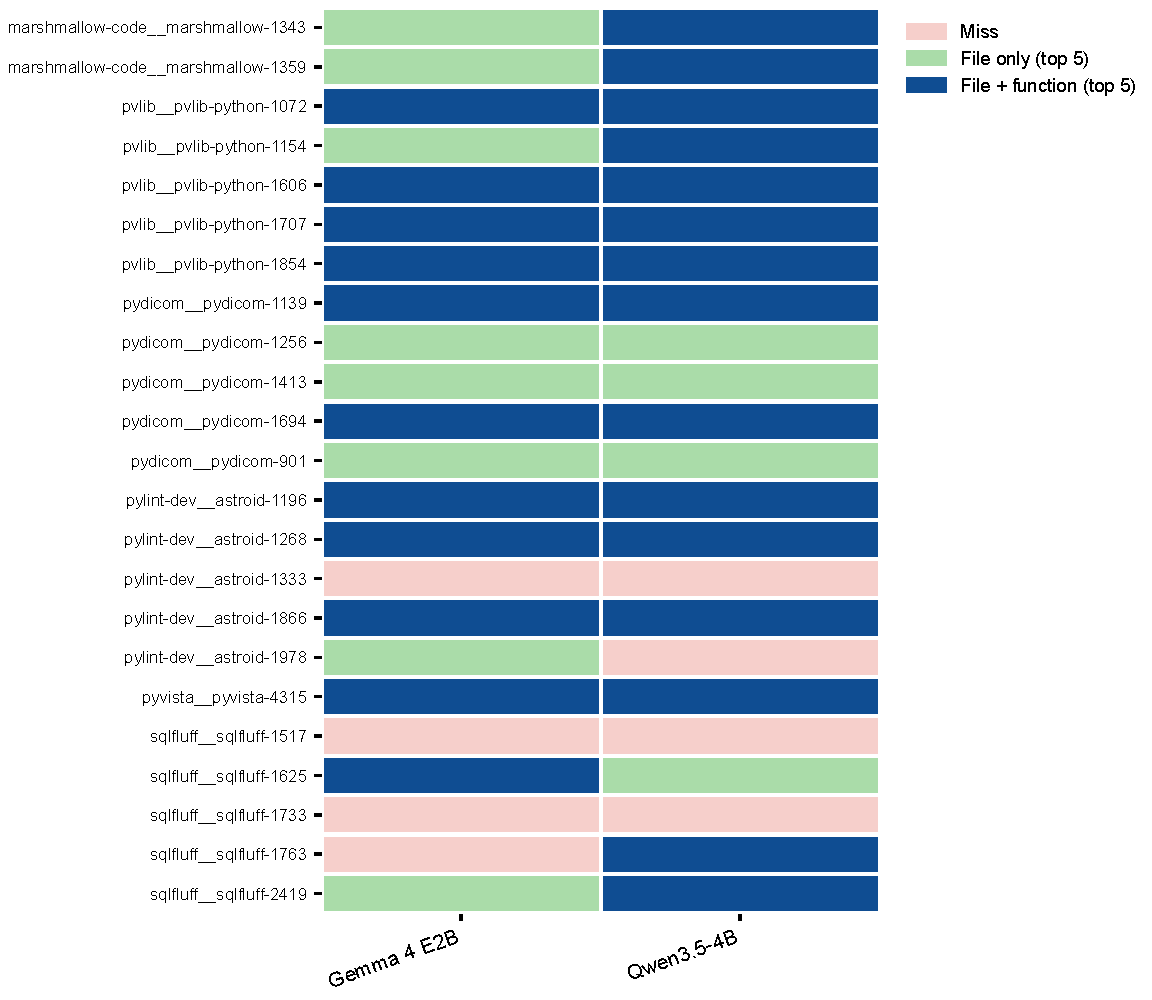
\includegraphics[width=0.24\textwidth]{2026-10-25_03_c1-dev/figures/outcomes.pdf}\hfill
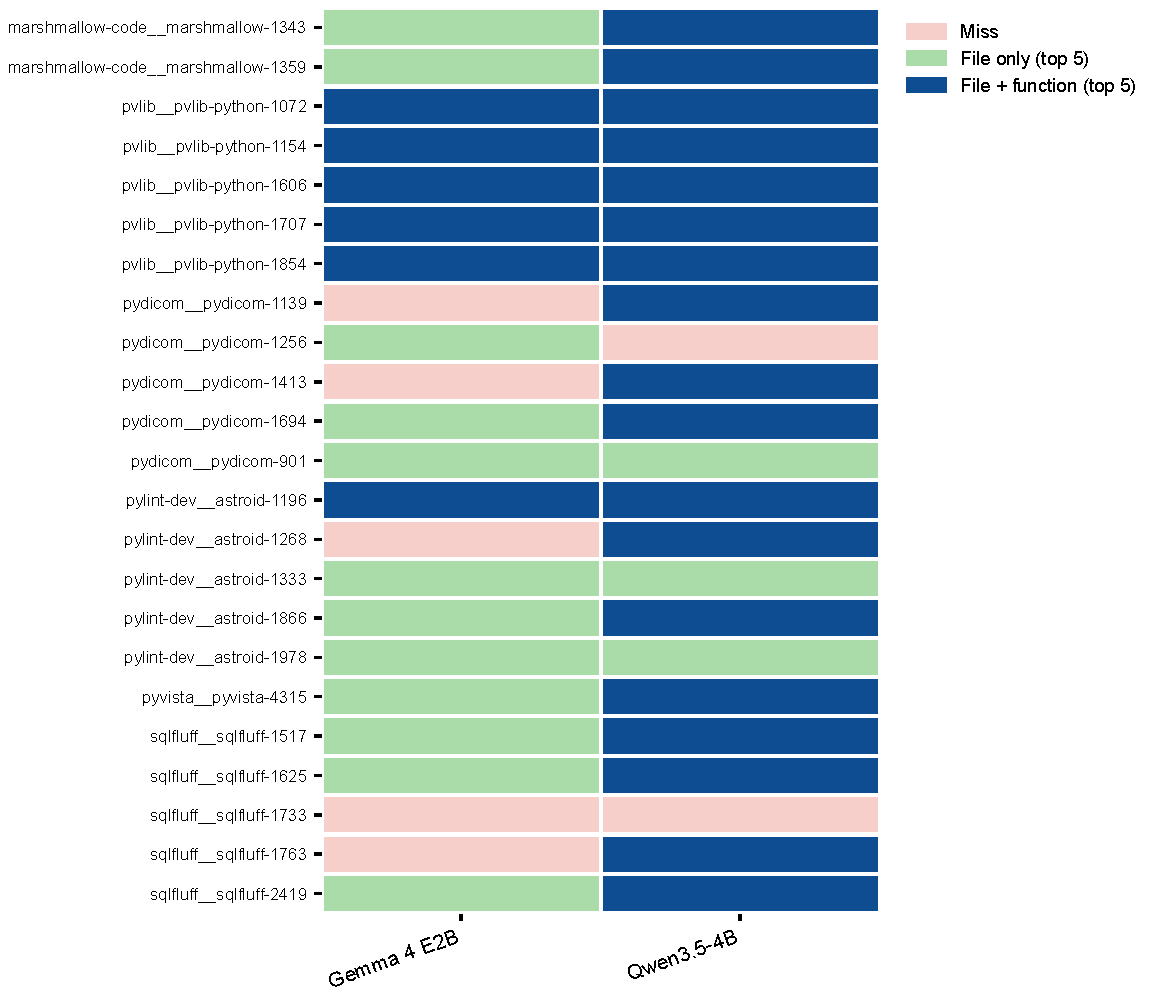
\includegraphics[width=0.24\textwidth]{2026-10-25_05_struct-dev/figures/outcomes.pdf}\hfill
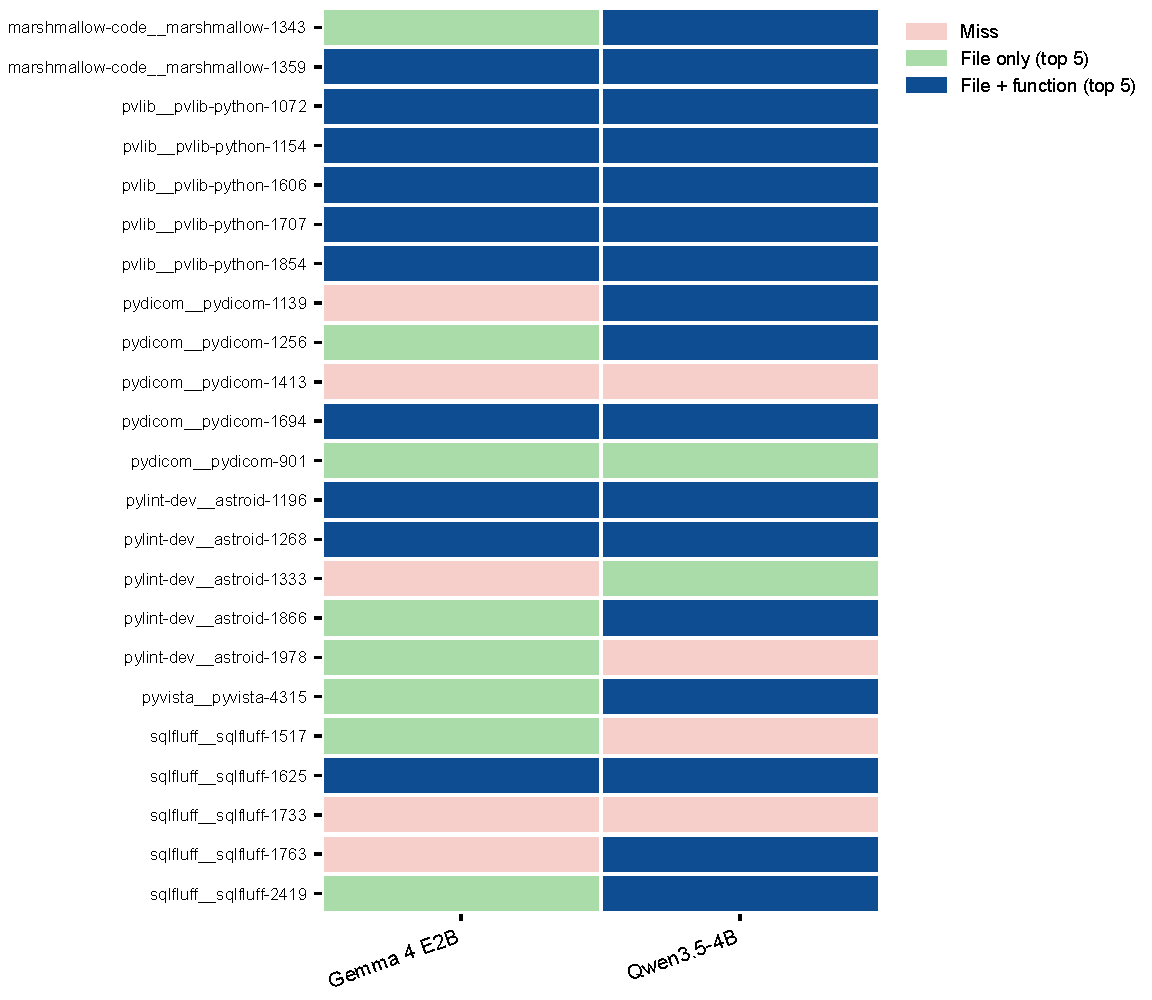
\includegraphics[width=0.24\textwidth]{2026-10-25_07_ranked-dev/figures/outcomes.pdf}\hfill
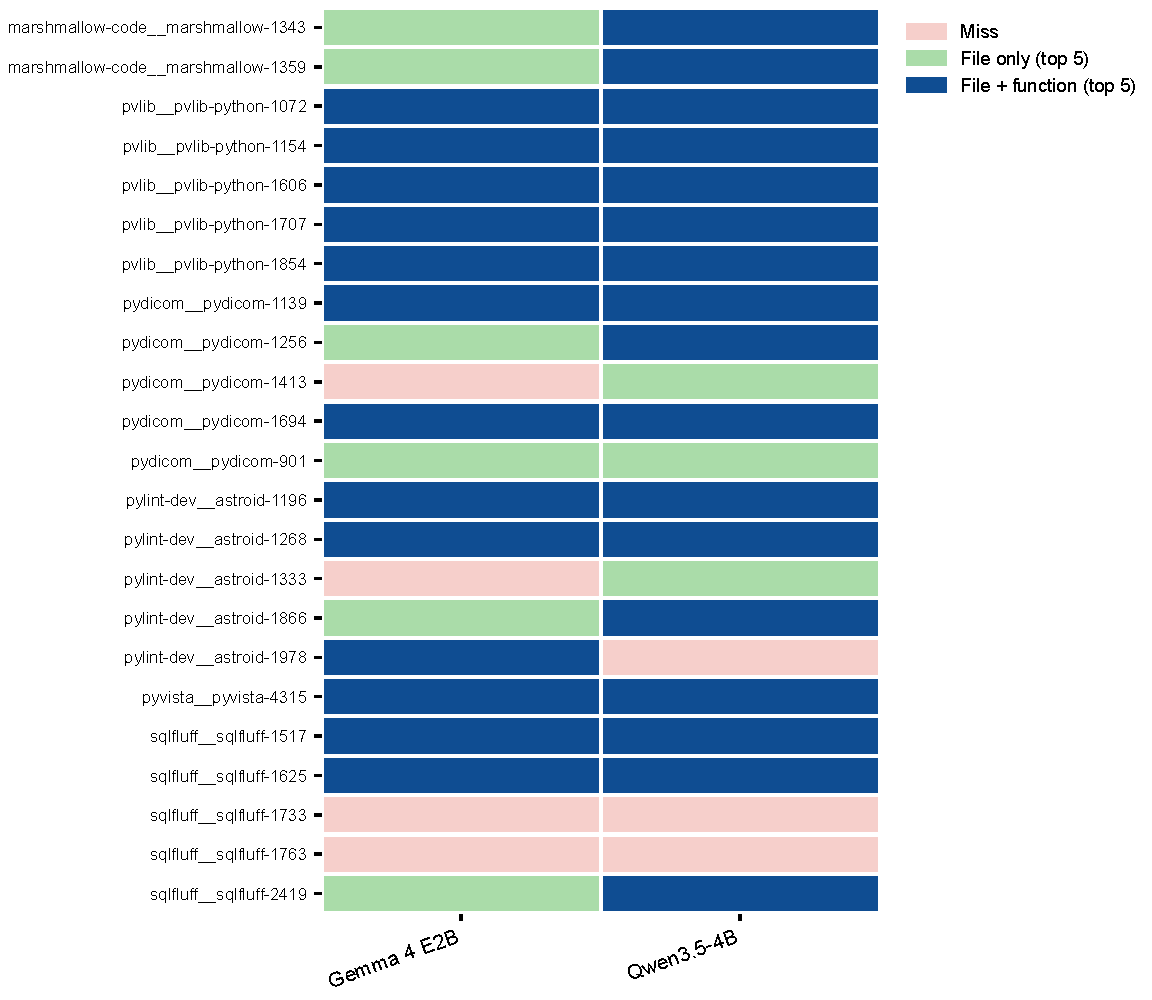
\includegraphics[width=0.24\textwidth]{2026-10-25_10_c2-dev/figures/outcomes.pdf}
\caption{\textbf{Per-task outcomes on the dev split} for experiments 03 (C1), 05 (structured answers), 07 (C1+H) and 10 (C2), left to right.}
\end{figure}
\begin{figure}[H]\centering
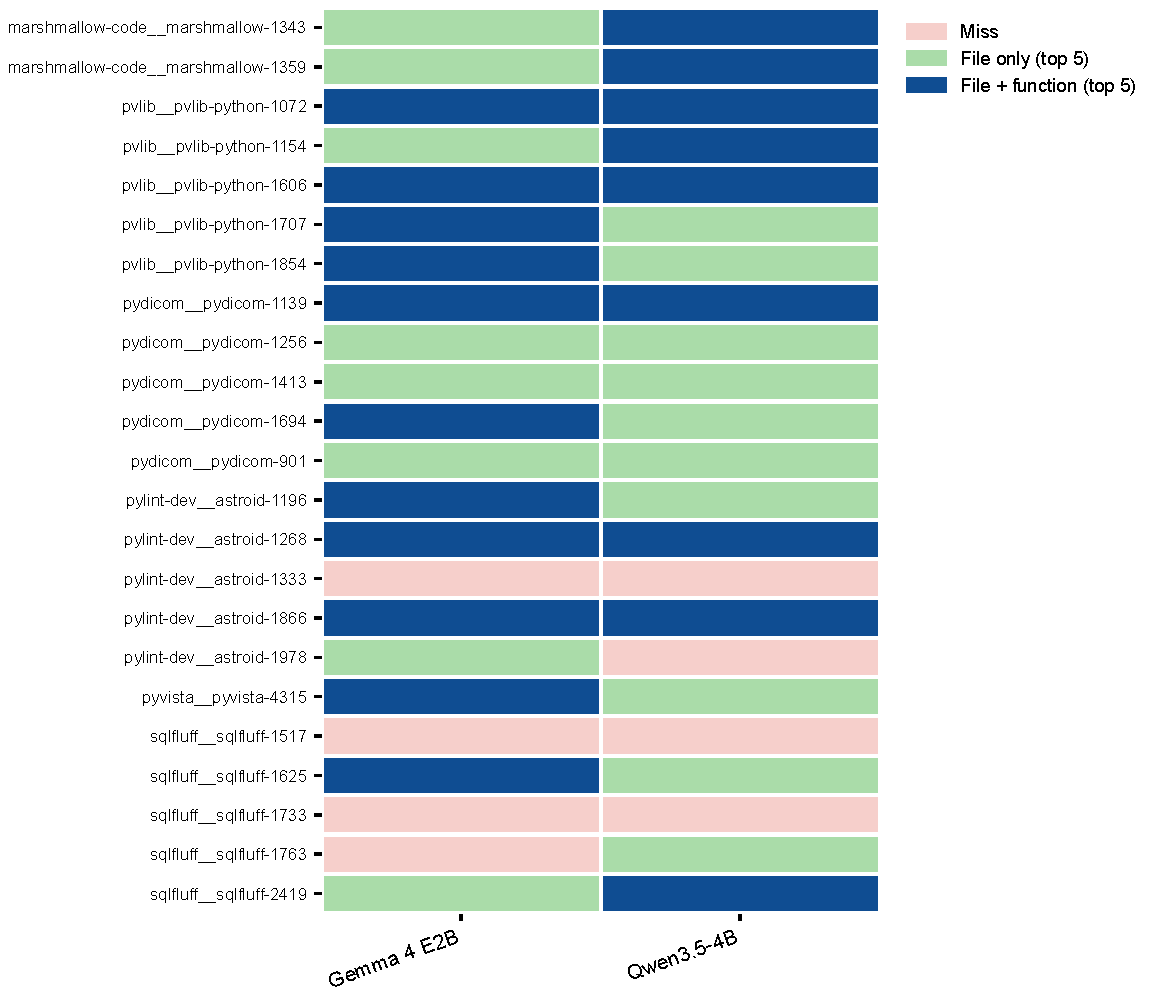
\includegraphics[width=0.24\textwidth]{2026-10-25_04_fmt-dev/figures/outcomes.pdf}\hfill
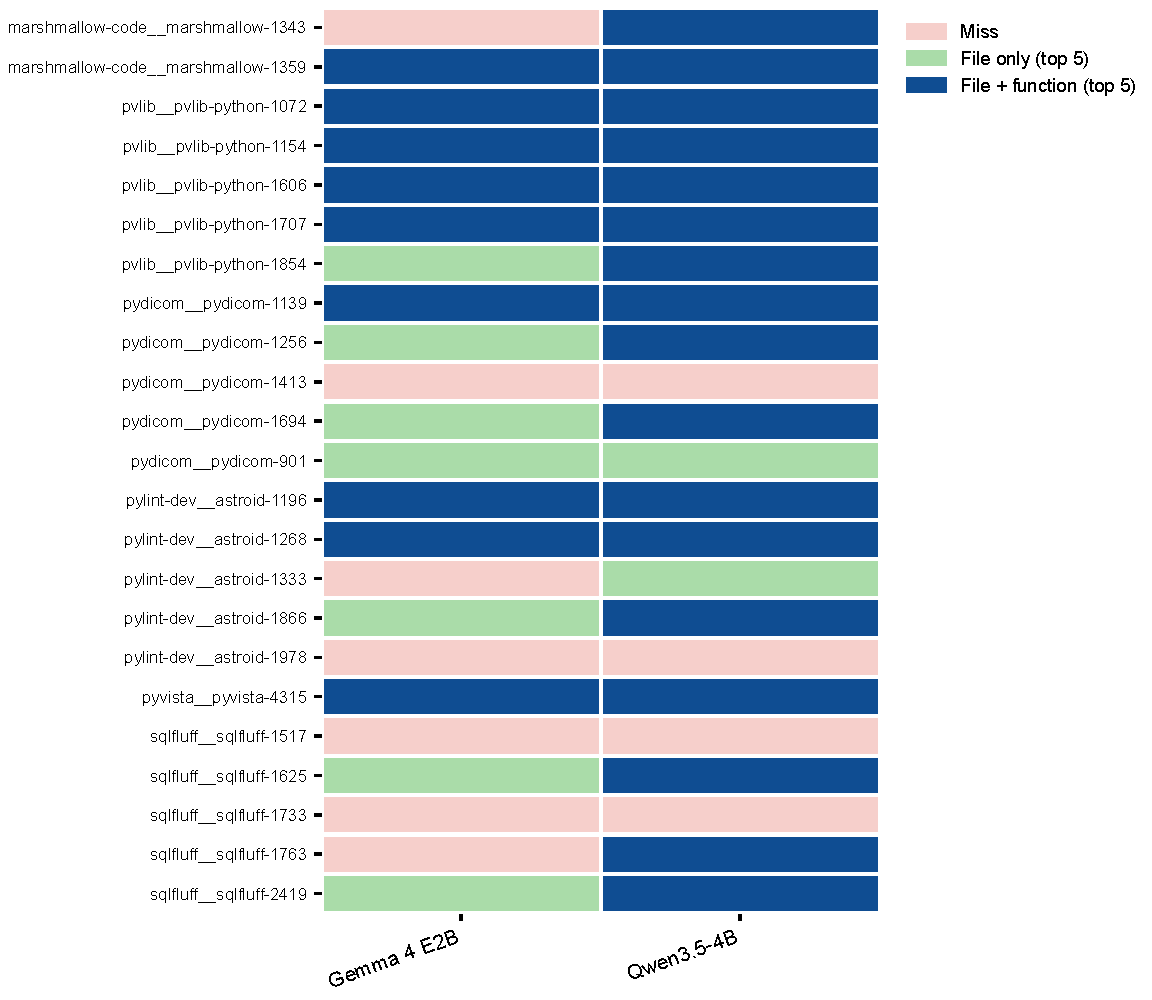
\includegraphics[width=0.24\textwidth]{2026-10-25_06_guard-dev/figures/outcomes.pdf}\hfill
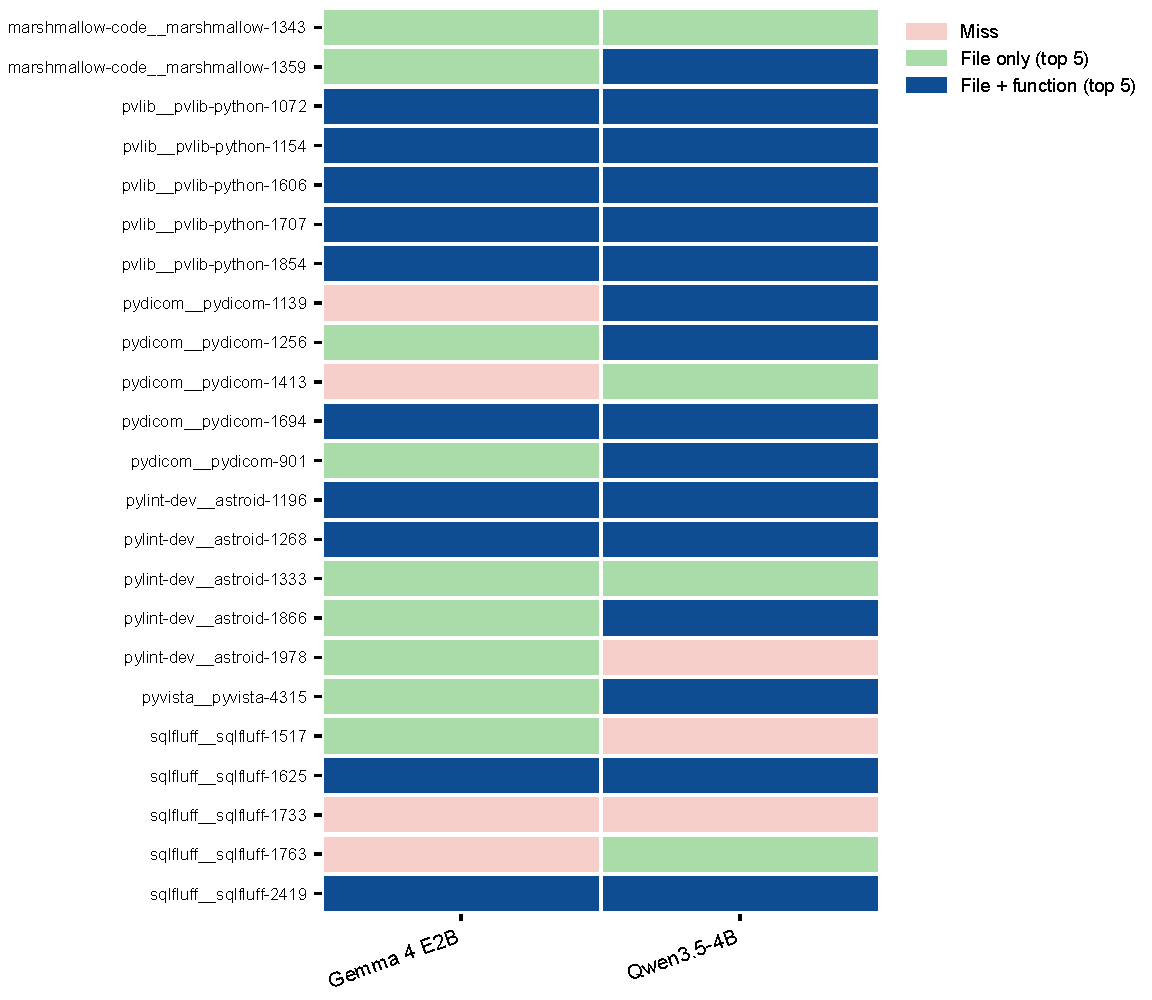
\includegraphics[width=0.24\textwidth]{2026-10-25_11_c3-dev/figures/outcomes.pdf}\hfill
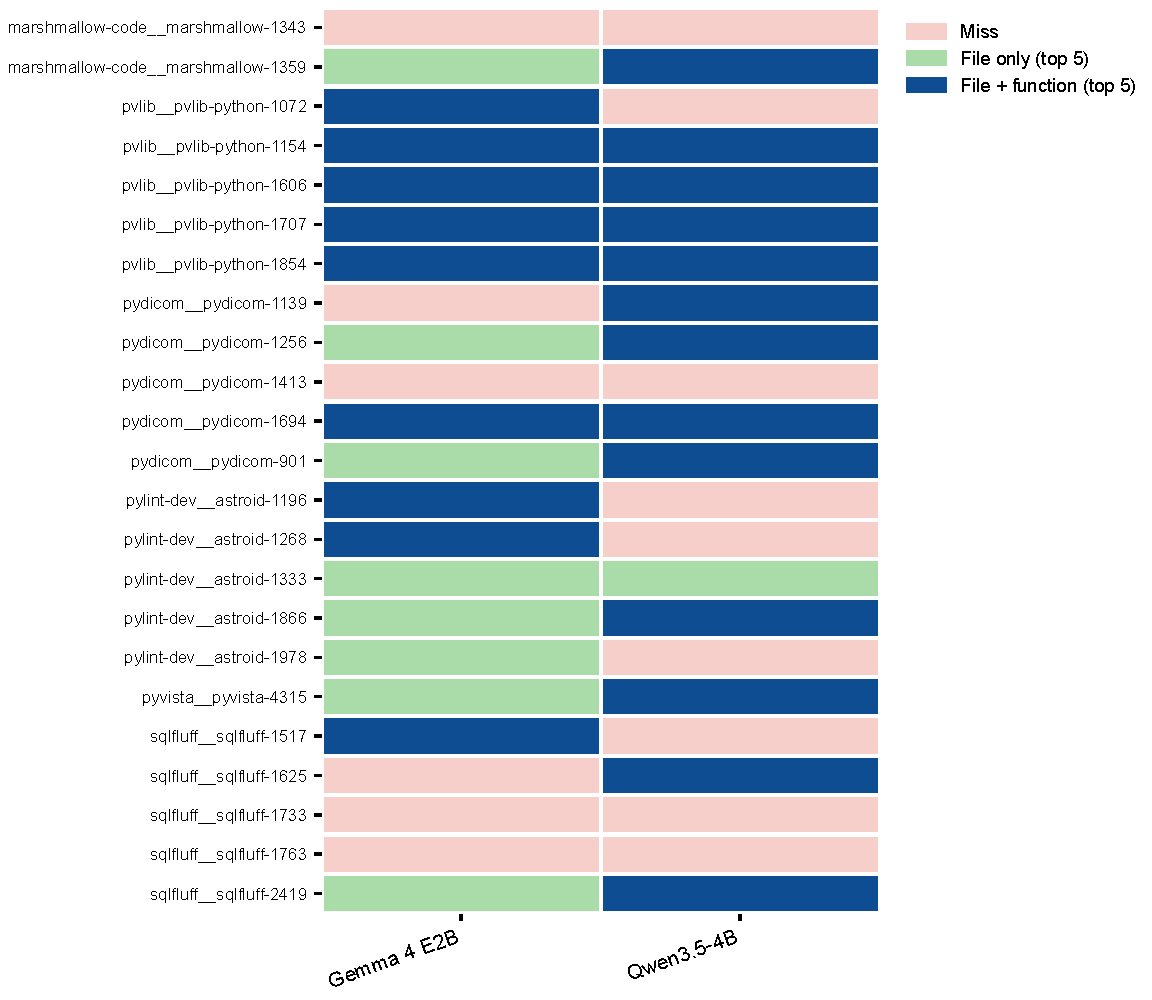
\includegraphics[width=0.24\textwidth]{2026-10-26_12_c4g-dev/figures/outcomes.pdf}
\caption{\textbf{Per-task outcomes on the dev split} for experiments 04 (regex names), 06 (guard and budget hints), 11 (C3) and 12 (C3 without grammar), left to right.}
\end{figure}
\expfig{2026-10-25_09_c0-dev/figures/outcomes.pdf}{\textbf{Per-task outcomes of BM25 on the dev split} (exp.\ 09).}{0.3}

\clearpage
\subsection{Test split}
\expfig{2026-10-26_13_c0-test/figures/summary.pdf}{\textbf{Exp.\ 13, C0 BM25 (test).} 33\% \fileone{}, 64\% \filefive{}, 36\% \funcfive{}, 47\% Function@10.}{0.92}
\expfig{2026-10-26_15_c1-test/figures/summary.pdf}{\textbf{Exp.\ 15, C1 (test).} \Gm{} hits the step limit in 72\% of episodes and repeats calls in 39\% of steps; 44\% of \Qw{}'s tasks contain malformed function names.}{0.92}
\expfig{2026-10-27_16_h07-test/figures/summary.pdf}{\textbf{Exp.\ 16, C1+H (test).} \Qw{} \funcfive{} 70\% (from 51\%); \Gm{}'s forced submissions fall to 9\%.}{0.92}
\expfig{2026-10-26_14_c2-test/figures/summary.pdf}{\textbf{Exp.\ 14, C2 (test), the full system.} \Qw{}: 85\% \fileone{}, 74\% \funcfive{}; \Gm{}: 66\% and 36\%.}{0.92}
\expfig{2026-11-09_17_c3-test/figures/summary.pdf}{\textbf{Exp.\ 17, C3 (test).} Every accuracy metric slightly lower than C2, with more generated tokens.}{0.92}
\expfig{2026-11-09_18_c4g-test/figures/summary.pdf}{\textbf{Exp.\ 18, C2 without grammar (test).} Invalid replies in 45\% (\Gm{}) and 79\% (\Qw{}) of episodes; 59\% of \Qw{}'s answers are empty.}{0.92}

\begin{figure}[H]\centering
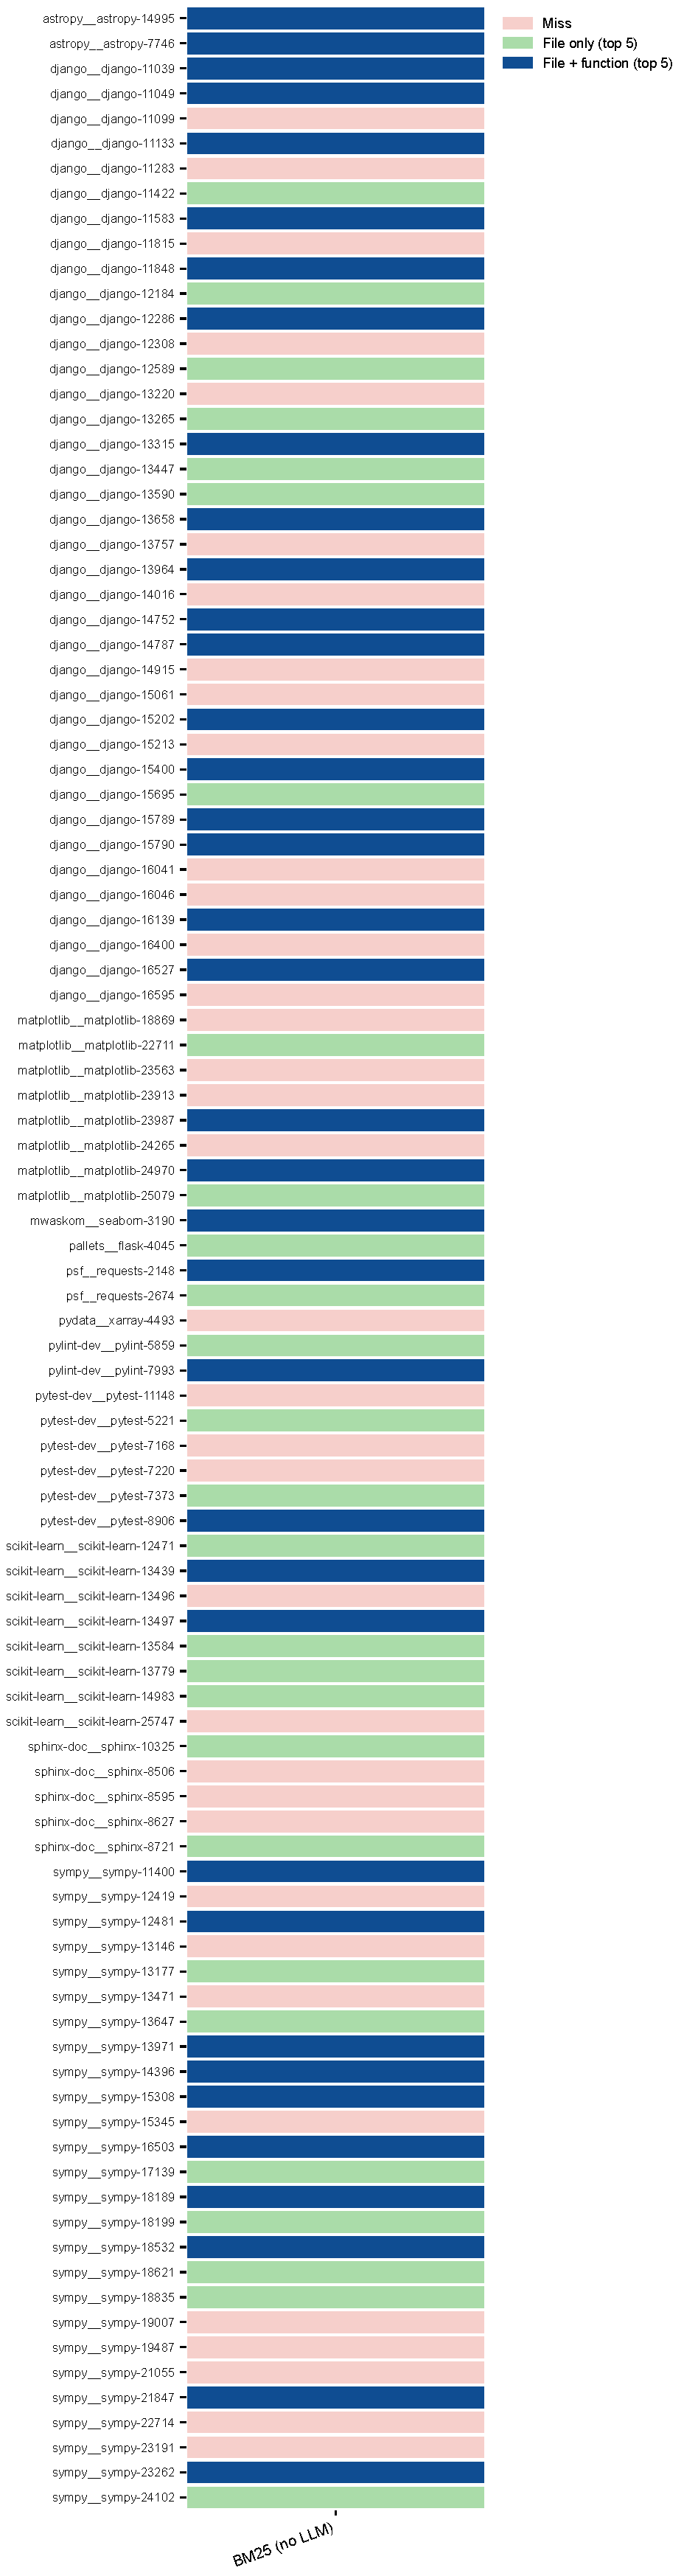
\includegraphics[height=0.74\textheight]{2026-10-26_13_c0-test/figures/outcomes.pdf}\hfill
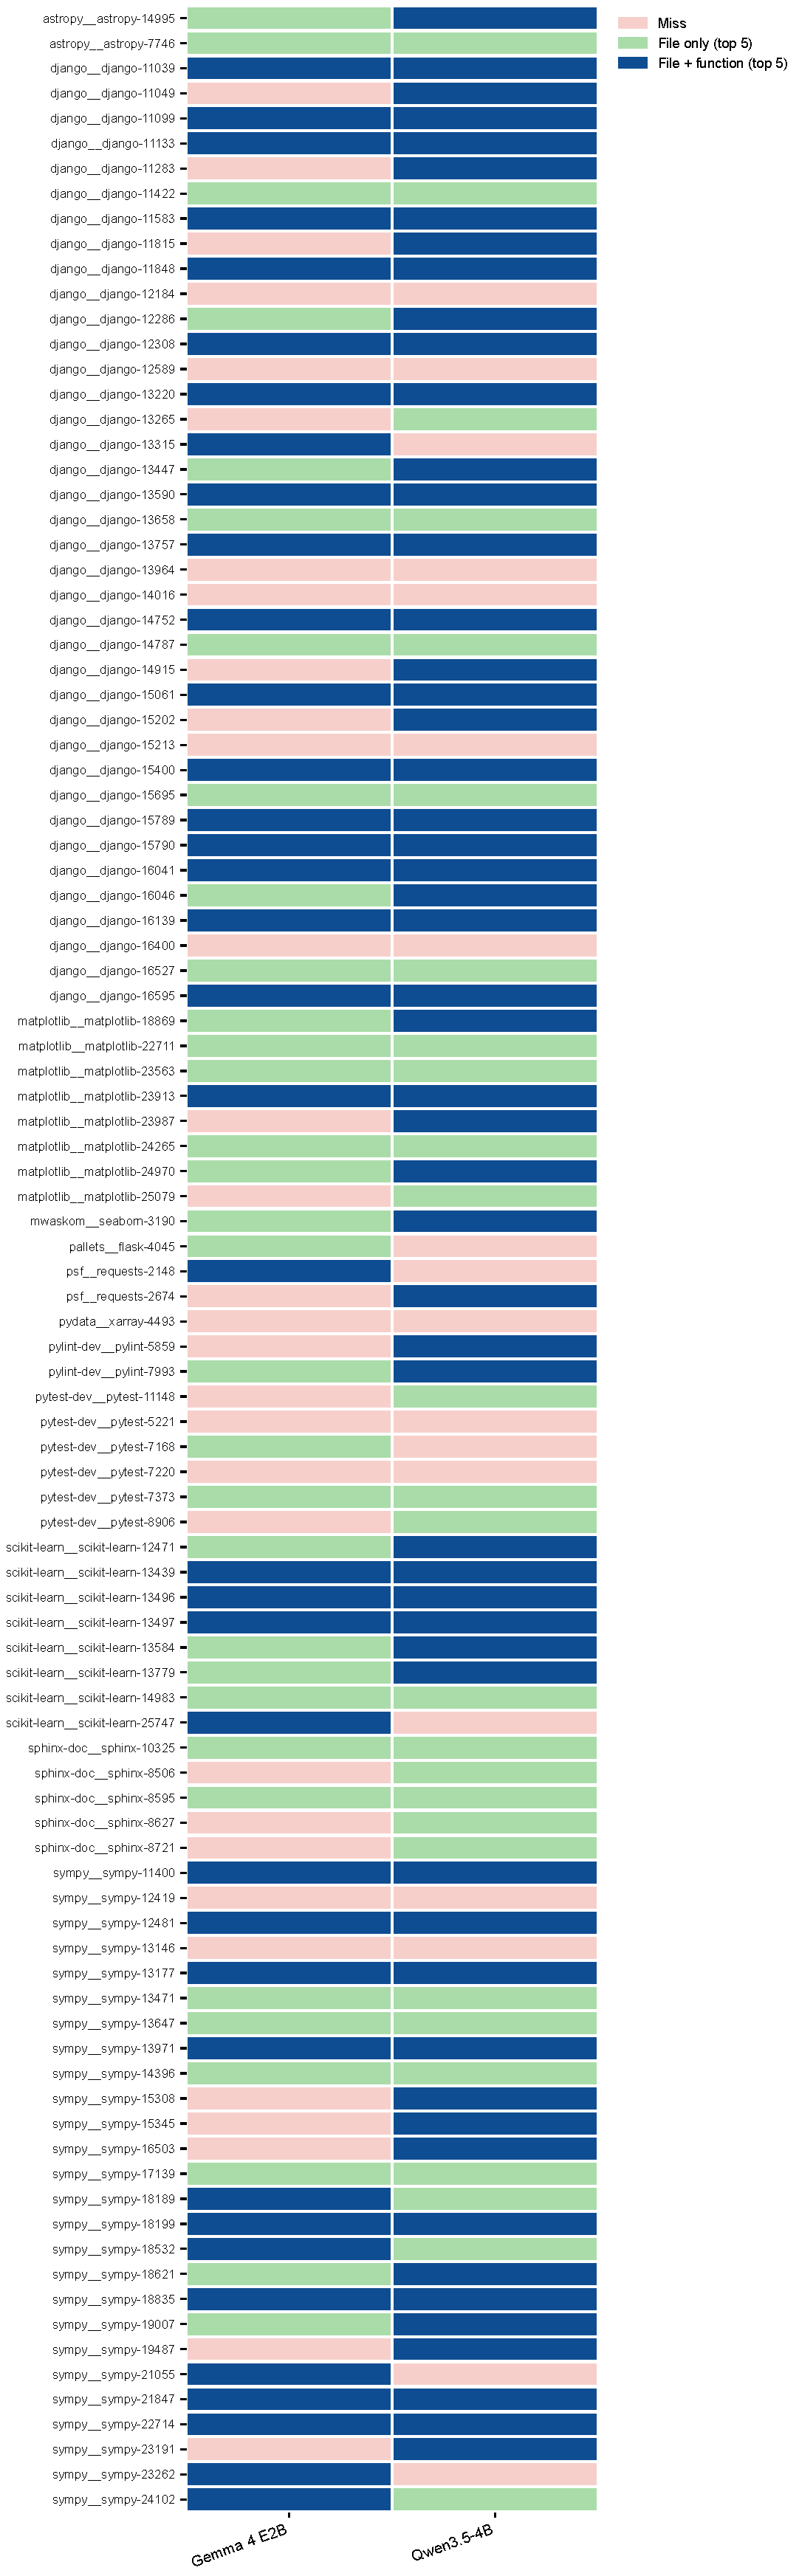
\includegraphics[height=0.74\textheight]{2026-10-26_15_c1-test/figures/outcomes.pdf}\hfill
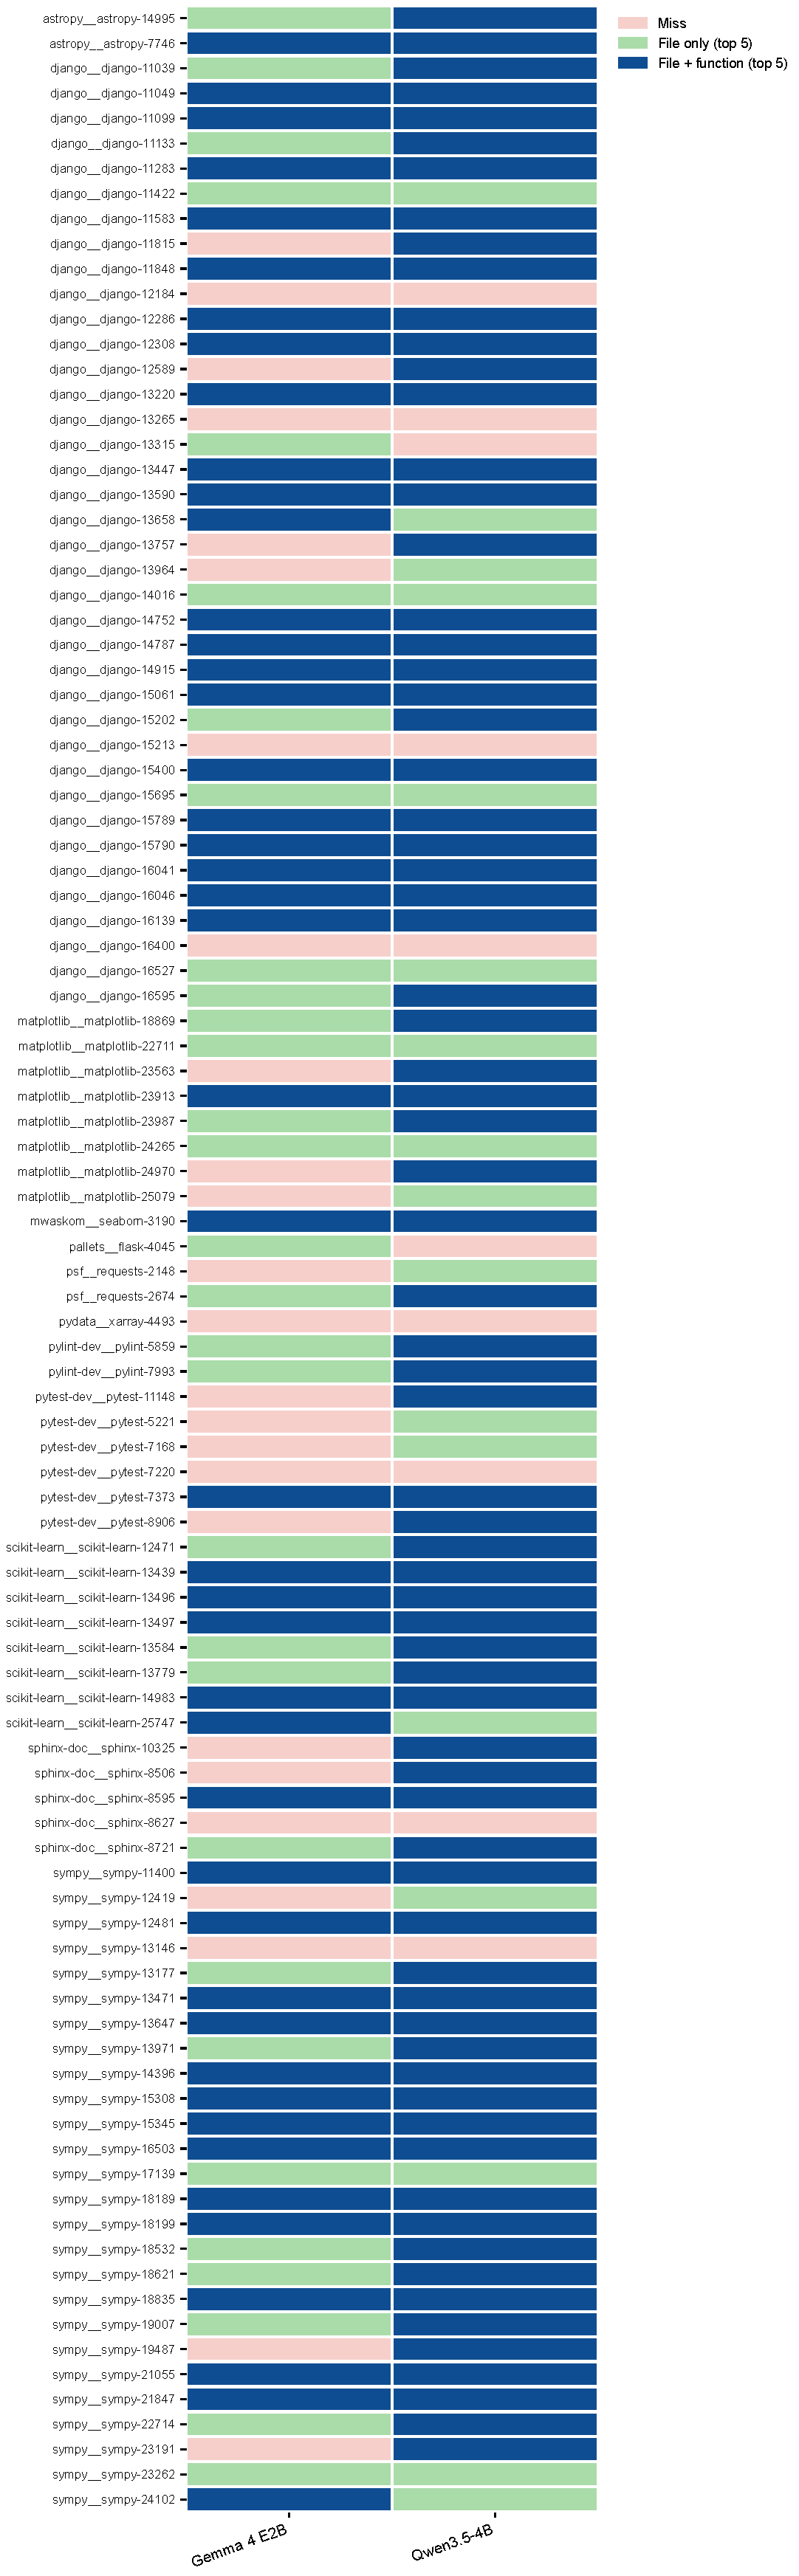
\includegraphics[height=0.74\textheight]{2026-10-27_16_h07-test/figures/outcomes.pdf}
\caption{\textbf{Per-task outcomes on the test subset}: C0 BM25 (exp.\ 13), C1 (exp.\ 15) and C1+H (exp.\ 16), left to right.}
\end{figure}
\begin{figure}[H]\centering
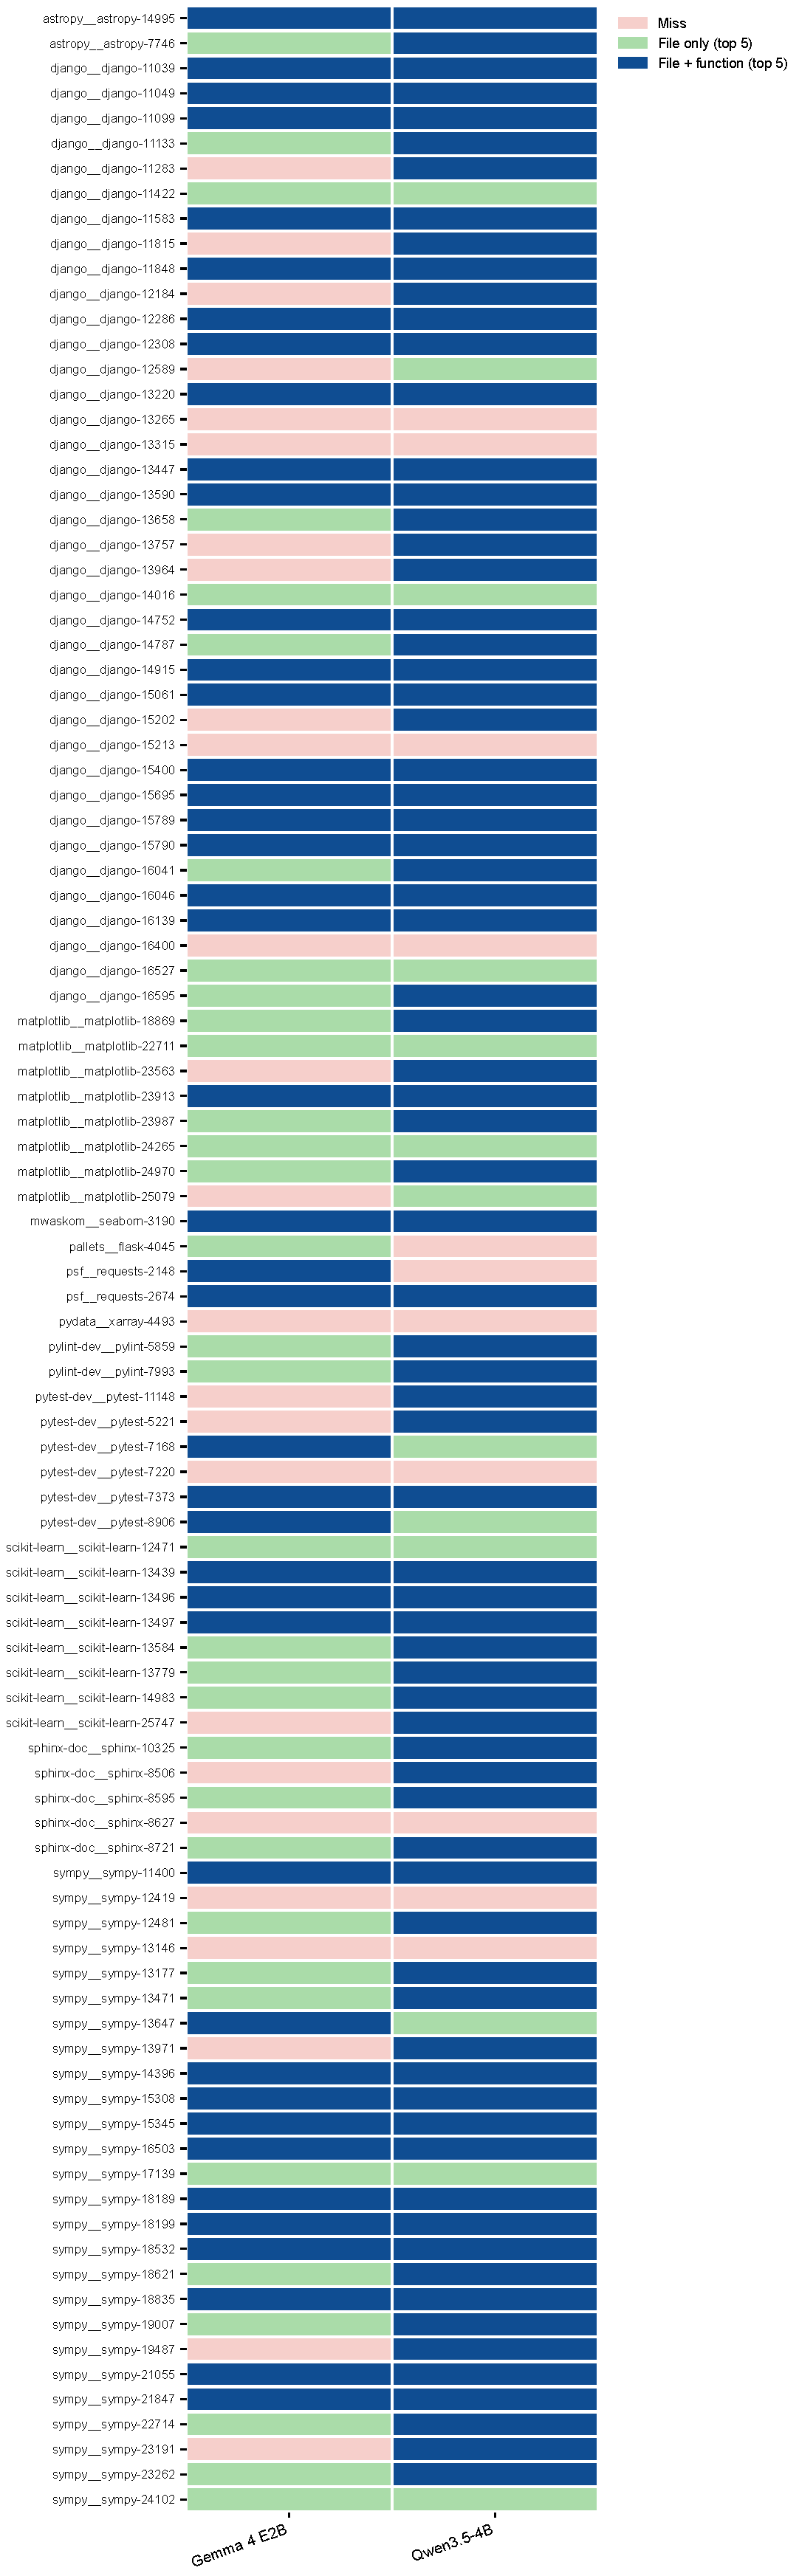
\includegraphics[height=0.74\textheight]{2026-10-26_14_c2-test/figures/outcomes.pdf}\hfill
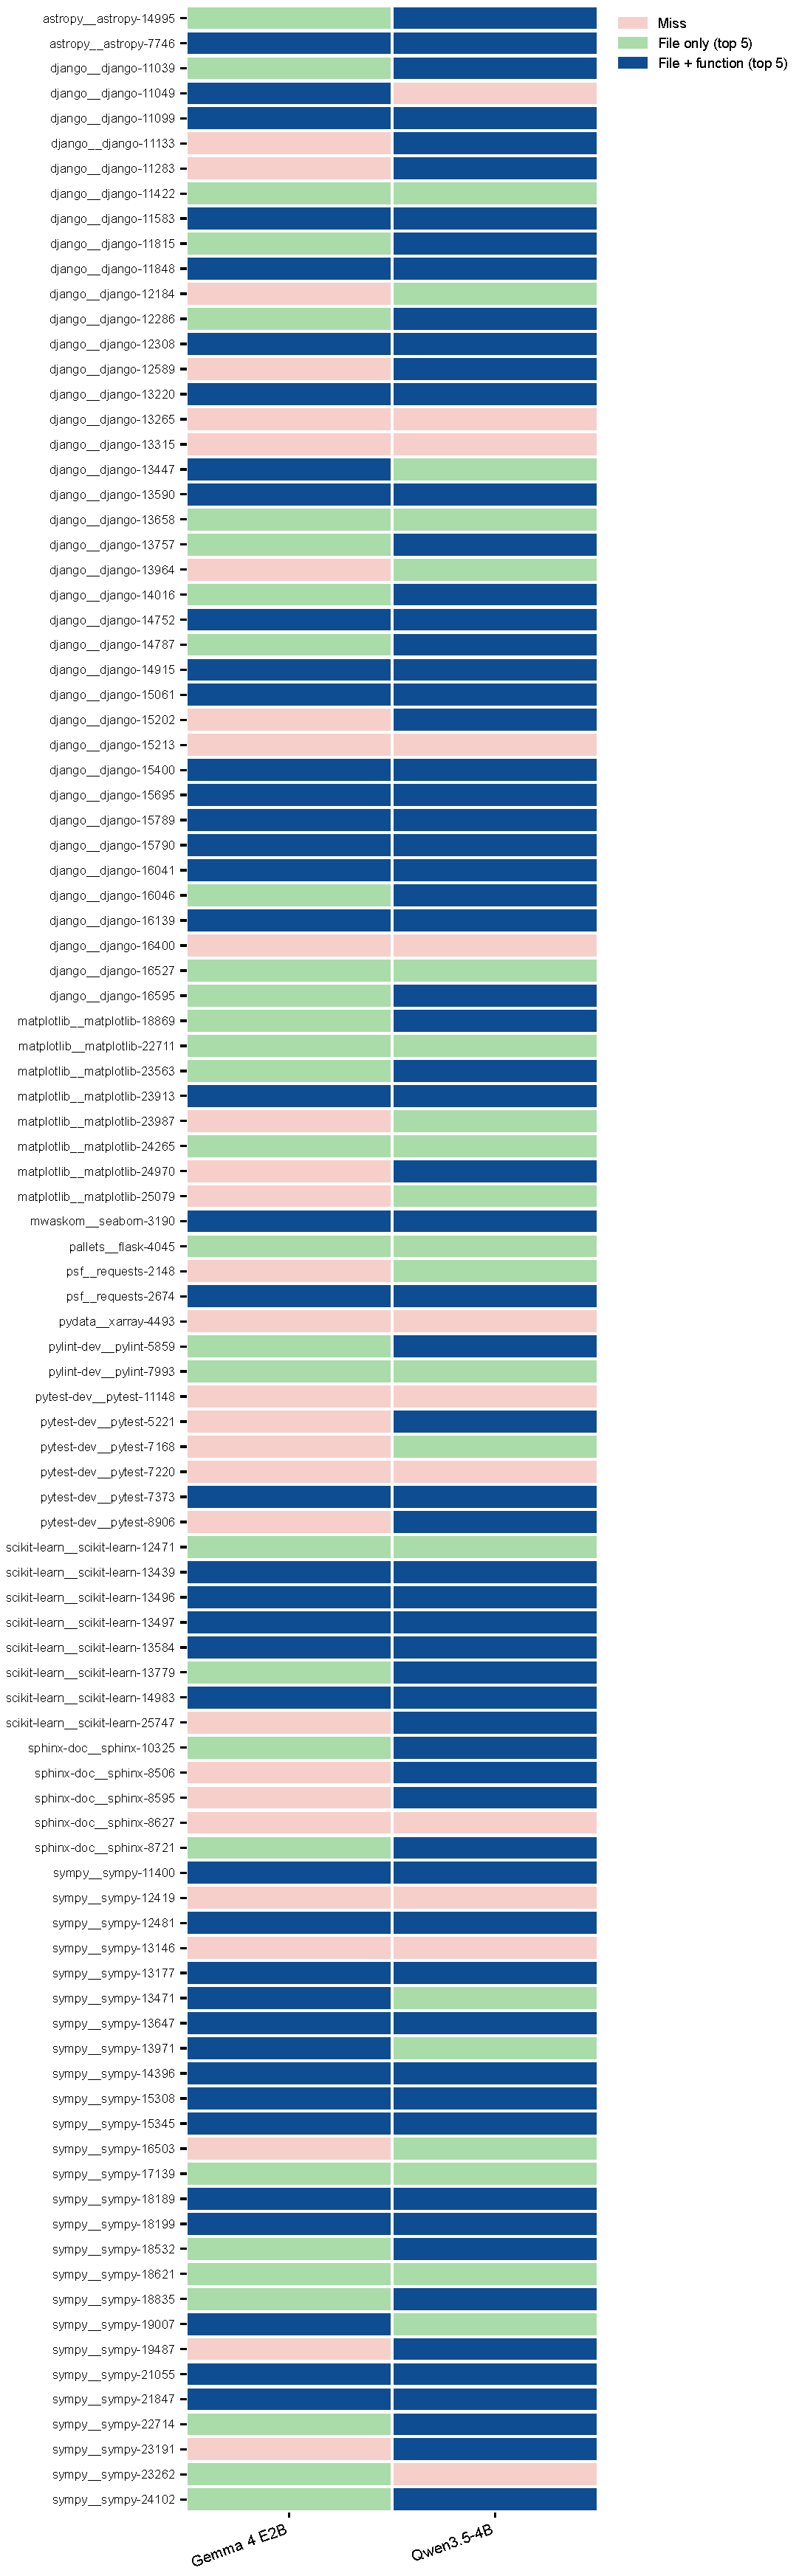
\includegraphics[height=0.74\textheight]{2026-11-09_17_c3-test/figures/outcomes.pdf}\hfill
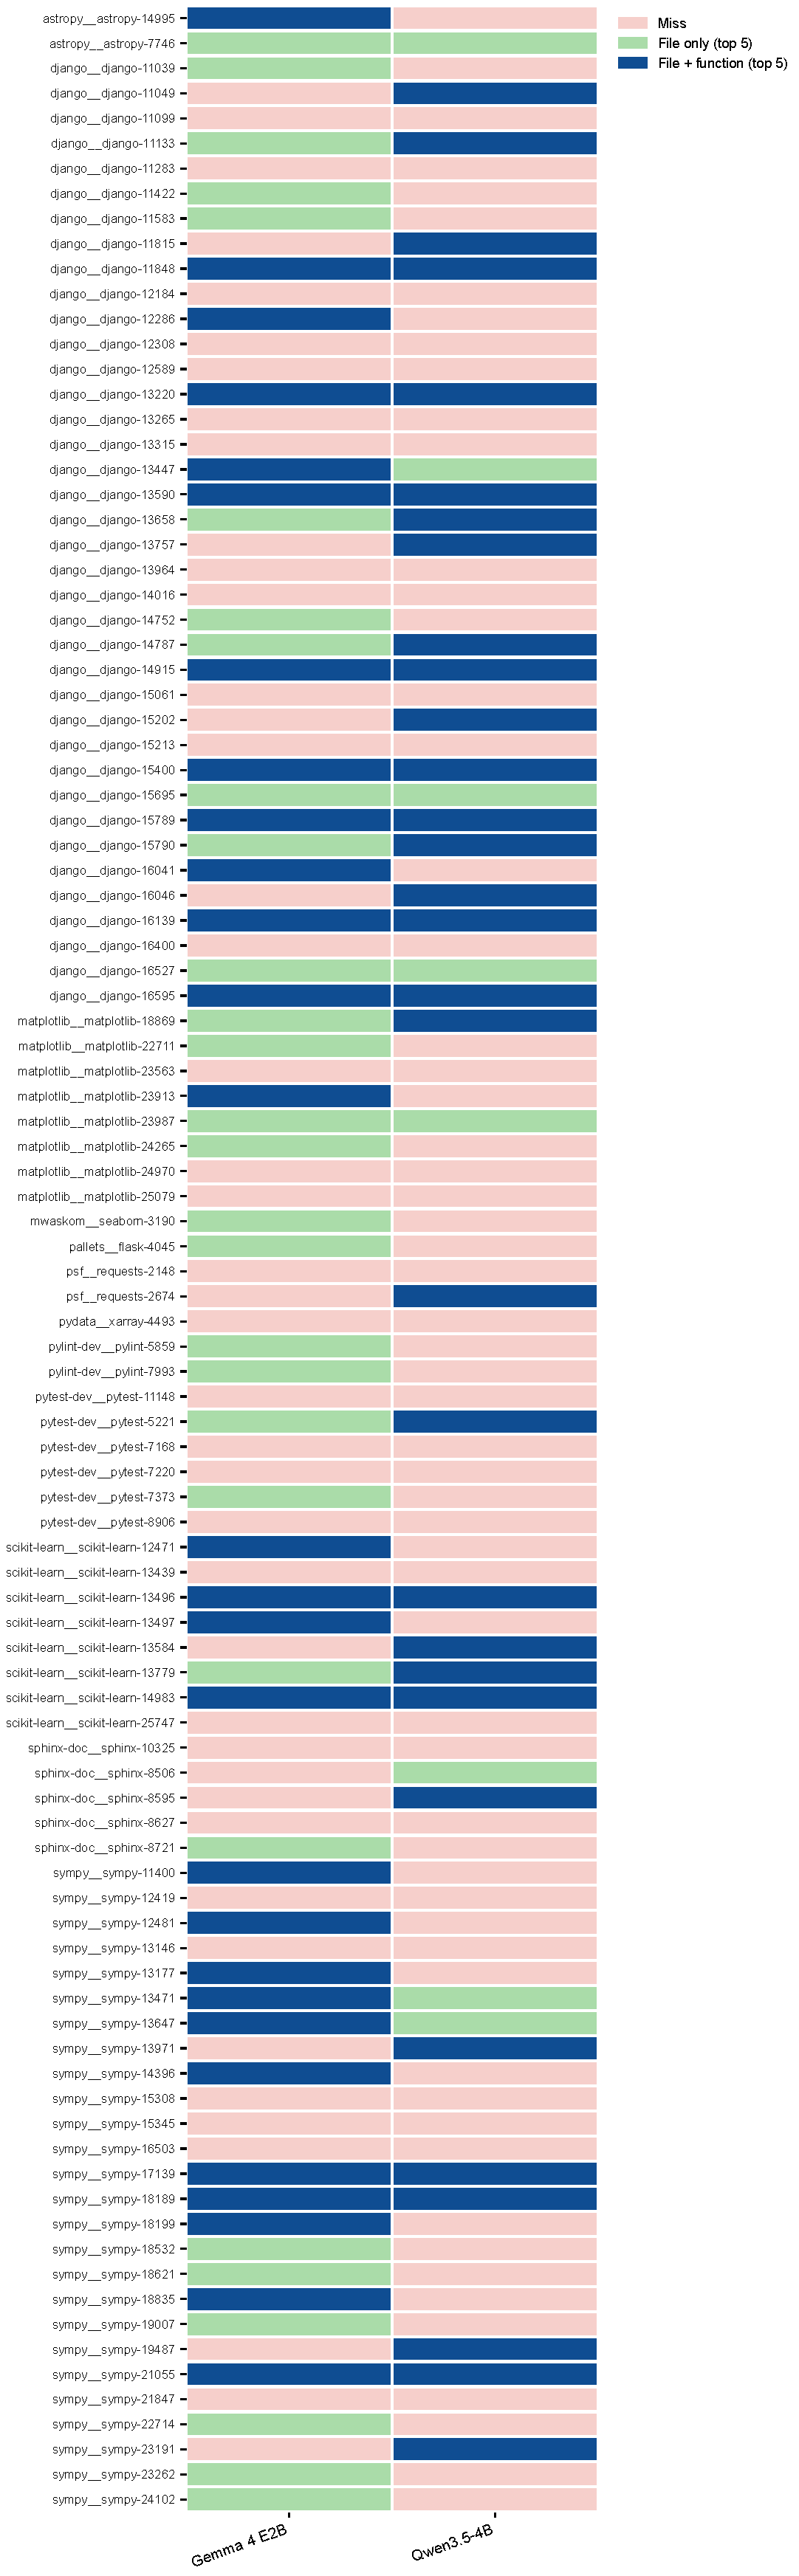
\includegraphics[height=0.74\textheight]{2026-11-09_18_c4g-test/figures/outcomes.pdf}
\caption{\textbf{Per-task outcomes on the test subset}: C2 (exp.\ 14), C3 (exp.\ 17) and C2 without grammar (exp.\ 18), left to right.}
\end{figure}

\end{document}
